\documentclass[11pt]{report}
\usepackage{float}
\usepackage{graphicx}
\usepackage{xcolor}
\usepackage[T1]{fontenc}
\usepackage{lmodern}
\usepackage{subcaption}
\usepackage{titlesec}
\usepackage[toc,page]{appendix}


\usepackage{listings}
\usepackage{hyperref}
 
\definecolor{dkgreen}{rgb}{0,0.6,0}
\definecolor{gray}{rgb}{0.5,0.5,0.5}
\definecolor{mauve}{rgb}{0.58,0,0.82}

\lstset{frame=tb,
  language=R,
  aboveskip=3mm,
  belowskip=3mm,
  showstringspaces=false,
  columns=flexible,
  basicstyle={\small\ttfamily},
  numbers=none,
  numberstyle=\tiny\color{gray},
  keywordstyle=\color{blue},
  commentstyle=\color{dkgreen},
  stringstyle=\color{mauve},
  breaklines=true,
  breakatwhitespace=true,
  tabsize=3
}
\usepackage[english]{babel}
\usepackage[utf8x]{inputenc}
\usepackage[numbers]{natbib}
\usepackage[a4paper, total={6in, 8in}]{geometry}

% fix the zero section
\renewcommand{\thesection}{\arabic{section}}


\begin{document}


\title{Data-Driven STEM Curriculum Design and Education with Association Graphs and Unsupervised Learning Techniques}
\author{Angel Sarmiento}
\date{December 1, 2021}
\maketitle

\section{Abstract}

\indent In this work,  a series of investigations involving Text Mining and Unsupervised learning techniques were developed and evaluated.  Through the use machine learning based analytics methods such as Multi-Dimensional Scaling (MDS) and Latent Dirichlet Allocation this project aimed to generate course-concept associations that can be pivotal in future course and curriculum design. The performance of machine learning and analytics in the field of Learning Analytics is widely known to be effective in online class structures. However this application will be applied to a primarily in-person University. This allows these methods to be applied to potentially better advise students in University coursework for their long term goals by alleviating the pressure of learning a vast set of concepts from courses in which they might only need a small fraction of. The focus on this project was the course catalog at Florida Polytechnic University, where Document-term matrices, course-concept association graphs, and dimensionality reduction methods were constructed to investigate the future of catalogue design,  by unifying courses by their text information.  The work generated reusable templates with open-source technologies for applying these methodologies across the entire catalog with dynamic package management for reproducibility. This can be used for further analysis for planning course work and catalogs, while pointing students toward important associations between their current coursework and weaknesses they may have in other concepts.  This work highlights the techniques described above, along with a case study of different distance methods and their ability to segment courses into groupings.  The insights gained from this research project will help drive future developments and iterations on the application to aid in the University's rapid development. 






\section{Introduction}

\hspace*{0.5cm} Learning Analytics is a field existing at the cross-section of machine-learning and data analytics with education. Many different techniques exist to leverage data from coursework or user interactions from multiple different user-types at universities and enable predictive or inferential capabilities. However, the implementation of these techniques are often overlooked or not offered by universities, which can result in problems. For instance, students that may join classes intended for a wider set of majors/programs tend to have differing levels of programming experience that result in bottlenecks in teaching and topics covered. 

For this, a network analysis of skills acquired in student’s previous coursework was investigated with a focus on creating concept-courses association graphs using a variety of distance metrics.  These distance metrics include cosine similarity,  Jaccard's index, Burrow's Delta, Argamon's Linear Delta and others \citep{lan_tag-aware_2014}\citep{lan_sparse_nodate}  that were implemented on Florida Polytechnic University course data, focusing on the contents in each course and the overlap of topics. 

\indent This technique was then used with dimensionality reduction techniques such as Multiple Correspondence Analysis (MCA) and MDS to generate biplots where possible clusters of concepts may be identified.  Initial focus was on the Data Science and Business Analytics curriculum, but can be broadened to include other plans of study once the methods are further developed. The investigation involved the concepts and methods described on both course descriptions and course outlines using both a bigram approach along with an approach using the full text passages of each respectively.  The final goal was to create reusable and reproducible templates for easy successive iterations. 




\section{Survey of Literature}



\indent Previous research work in Learning Analytics (LA) involve everything from surveys of machine learning techniques in developing education platforms, to novel statistical methods in data-driven education. Methods typically form solutions from predictive models estimating student performance on examinations and clustering models between students and questions \cite{barbu_data_nodate}. Some applications of these methods incorporate user modeling, identifying professors, students, and other faculty in relation to coursework as well as how they engage with online systems to provide insight to analytical platforms. LA typically focuses on the educational challenge while Educational Data Mining (EDM) focuses on developing algorithms and/or models \citep{hilliger_evaluating_2019}.

\indent Most applications make use of publicly available datasets \citep{romero_educational_2020} or data obtained from the relevant research university in which the study takes place. This enables peer review and rapid iteration of numerous machine learning and analytical concepts across different universities \citep{barbu_data_nodate}\citep{romero_educational_2020}\citep{hilliger_evaluating_2019}.  Specific data about users is typically obtained when the course in question is fully online or a Massively Open Online Course (MOOC). Work in this field has culminated in massive open source projects and publicly available work such as MIT’s Mapping Lab and even student-driven applications like MIT Crosslinks \citep{willcox_network_2017}. In these endeavors, MIT makes use of network modeling,  factor analysis, and machine learning techniques to create a robust ecosystem of tools to aid education at the institution. 

Dimensionality reduction methods like Multi-Dimensional Scaling (MDS) \citep{jjs} and Correspondence Analysis are used to generate latent space representations of the dynamics present in text data by utilizing distance metrics and the Singular Value Decomposition (SVD) respectively.  MDS allows for dynamic exploration of different distance metrics for use with text data, some of which are highly robust to features of text data.  Correspondence Analysis uses SVD to get latent space representations of text data,  where the new corresponding dimensions decrease successively in proportion of variance explained. 

\indent Novel methods like Sparse Factor analysis, introduced by A.S. Lan, et al. enhance previous work done in the field of LA, enabling question-concept association graphs to be generated. Different from the approach discussed in this proposal, question-concept associations allow a bank of questions to be linked by overarching concepts pertaining to a number of different courses, aligning students with possible avenues to make up shortcomings from missing fundamental concepts \citep{lan_sparse_nodate}\citep{willcox_network_2017}. Sparse Factor analysis takes the approach of a normal factor analysis, abstracting conceptual knowledge of learners and constructing association graphs, giving insight to their relationships. In the sparse case however, each question measures the learner’s knowledge on only a few concepts, resulting in a sparse questions-concept association matrix.  See Figure \ref{fig:sparfa}. This approach, while originally applied to the question-concept association level, is also applicable to the course-concept association level discussed here. 




\begin{figure}[ht]
\centering

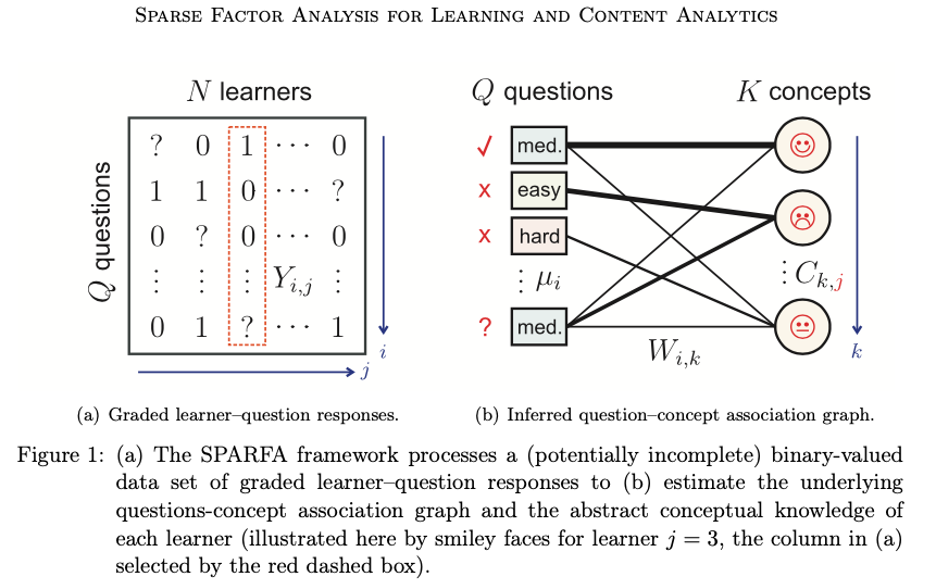
\includegraphics[width = \textwidth]{../images/sparfa.png}
\caption{Sparse Factor Analysis from the paper by A.S. Lan et. al, \citep{lan_tag-aware_2014}} \textit{Tag-Aware Ordinal Sparse Factor Analysis for Learning and Content Analytics}. Applied at the questions-concept association level but applicable to the more macro course-concept association level
\label{fig:sparfa}
\end{figure}



\indent The work here focused on the implementation of association graphs, unsupervised learning, and associated techniques, as well as the effectiveness of these methods in segmenting the course-concept associations present by validating with faculty at Florida Polytechnic University.

\section{Methodology of the Proposed Research Work}

This work starts with the collection of University course information from the entire course catalog at Florida Polytechnic University.  This provided, courses, concepts, plans of study, number of credits, and course descriptions. Once retrieved, a document-term matrix was created with rows representing topics, and columns representing the course where the word/bigram appears. This matrix was used in a dimensionality reduction method such as Multiple Correspondence Analysis (MCA) to generate biplots where clusters of topics can be identified. A process for a network analysis was then created to allow for instructions to provide examples of interest for all levels of proficiency and background. This process created a concept-courses association graph that can be used as a measure for verifying connections across topics/questions. This can enable incremental learning through successive iterations. 

\section{The Interdisciplinary Nature of the Proposed Research}

The use of machine learning and data science techniques to develop a  “Learning Analytics” tool not only affects computer science related fields of education but can be applied to all fields in STEM/non-STEM education. Course-concept associations can be developed not only within fields but across disciplines, enabling flexible coursework for students that are tangentially aligned with the topics of a class (E.g. Computer science students needing Differential Equations as a background for a Scientific Computation class, which involves the computation of a numerical solution). Other interdisciplinary areas are information retrieval, recommender systems, social network analysis, document-driven data mining, cognitive psychology, and others. The methods described here are applicable to any degree program or course catalogs. 





\section{Specific Objectives and Goals}

The objective of this research project was to develop a useful tool/application implementing learning analytics that can be upscaled to the needs of Florida Polytechnic University as it grows. This involves implementing robust text mining and network analysis algorithms that can be embedded within templates for expanding the university course catalog and dynamically applying these methods across degrees. 

\section{Results}

There were a few primary deliverables expected from the investigations associated with this project. We were able to 
identify a difference in course-concepts to the “classic” catalog that is validated by professors teaching in the DSBA 
curriculum. Evaluation was done in the form of tests of the proof of concept and the viability of the methods described.  
The templates apply the different methods to both course descriptions and course outlines. The data was cleaned using 
regular expressions \citep{regex} and text mining techniques like the creation of bigrams, the removal of stop words 
(the, a, and, etc.) and other data cleaning techniques.  An open source repository containing all materials, libraries, 
code, and educational documentation available on GitHub was developed and maintained for future developers to have more 
insight on the methodology utilized here to hopefully be iterated on in future versions of the project.  
 \href{https://github.com/angel-sarmiento/sparse-learning-analytics}{\textbf{The direct link to this repository can be found here}} 
  and Figure \ref{fig:repo} shows the repository (https://github.com/angel-sarmiento/sparse-learning-analytics).  

\begin{figure}[H]
\centering

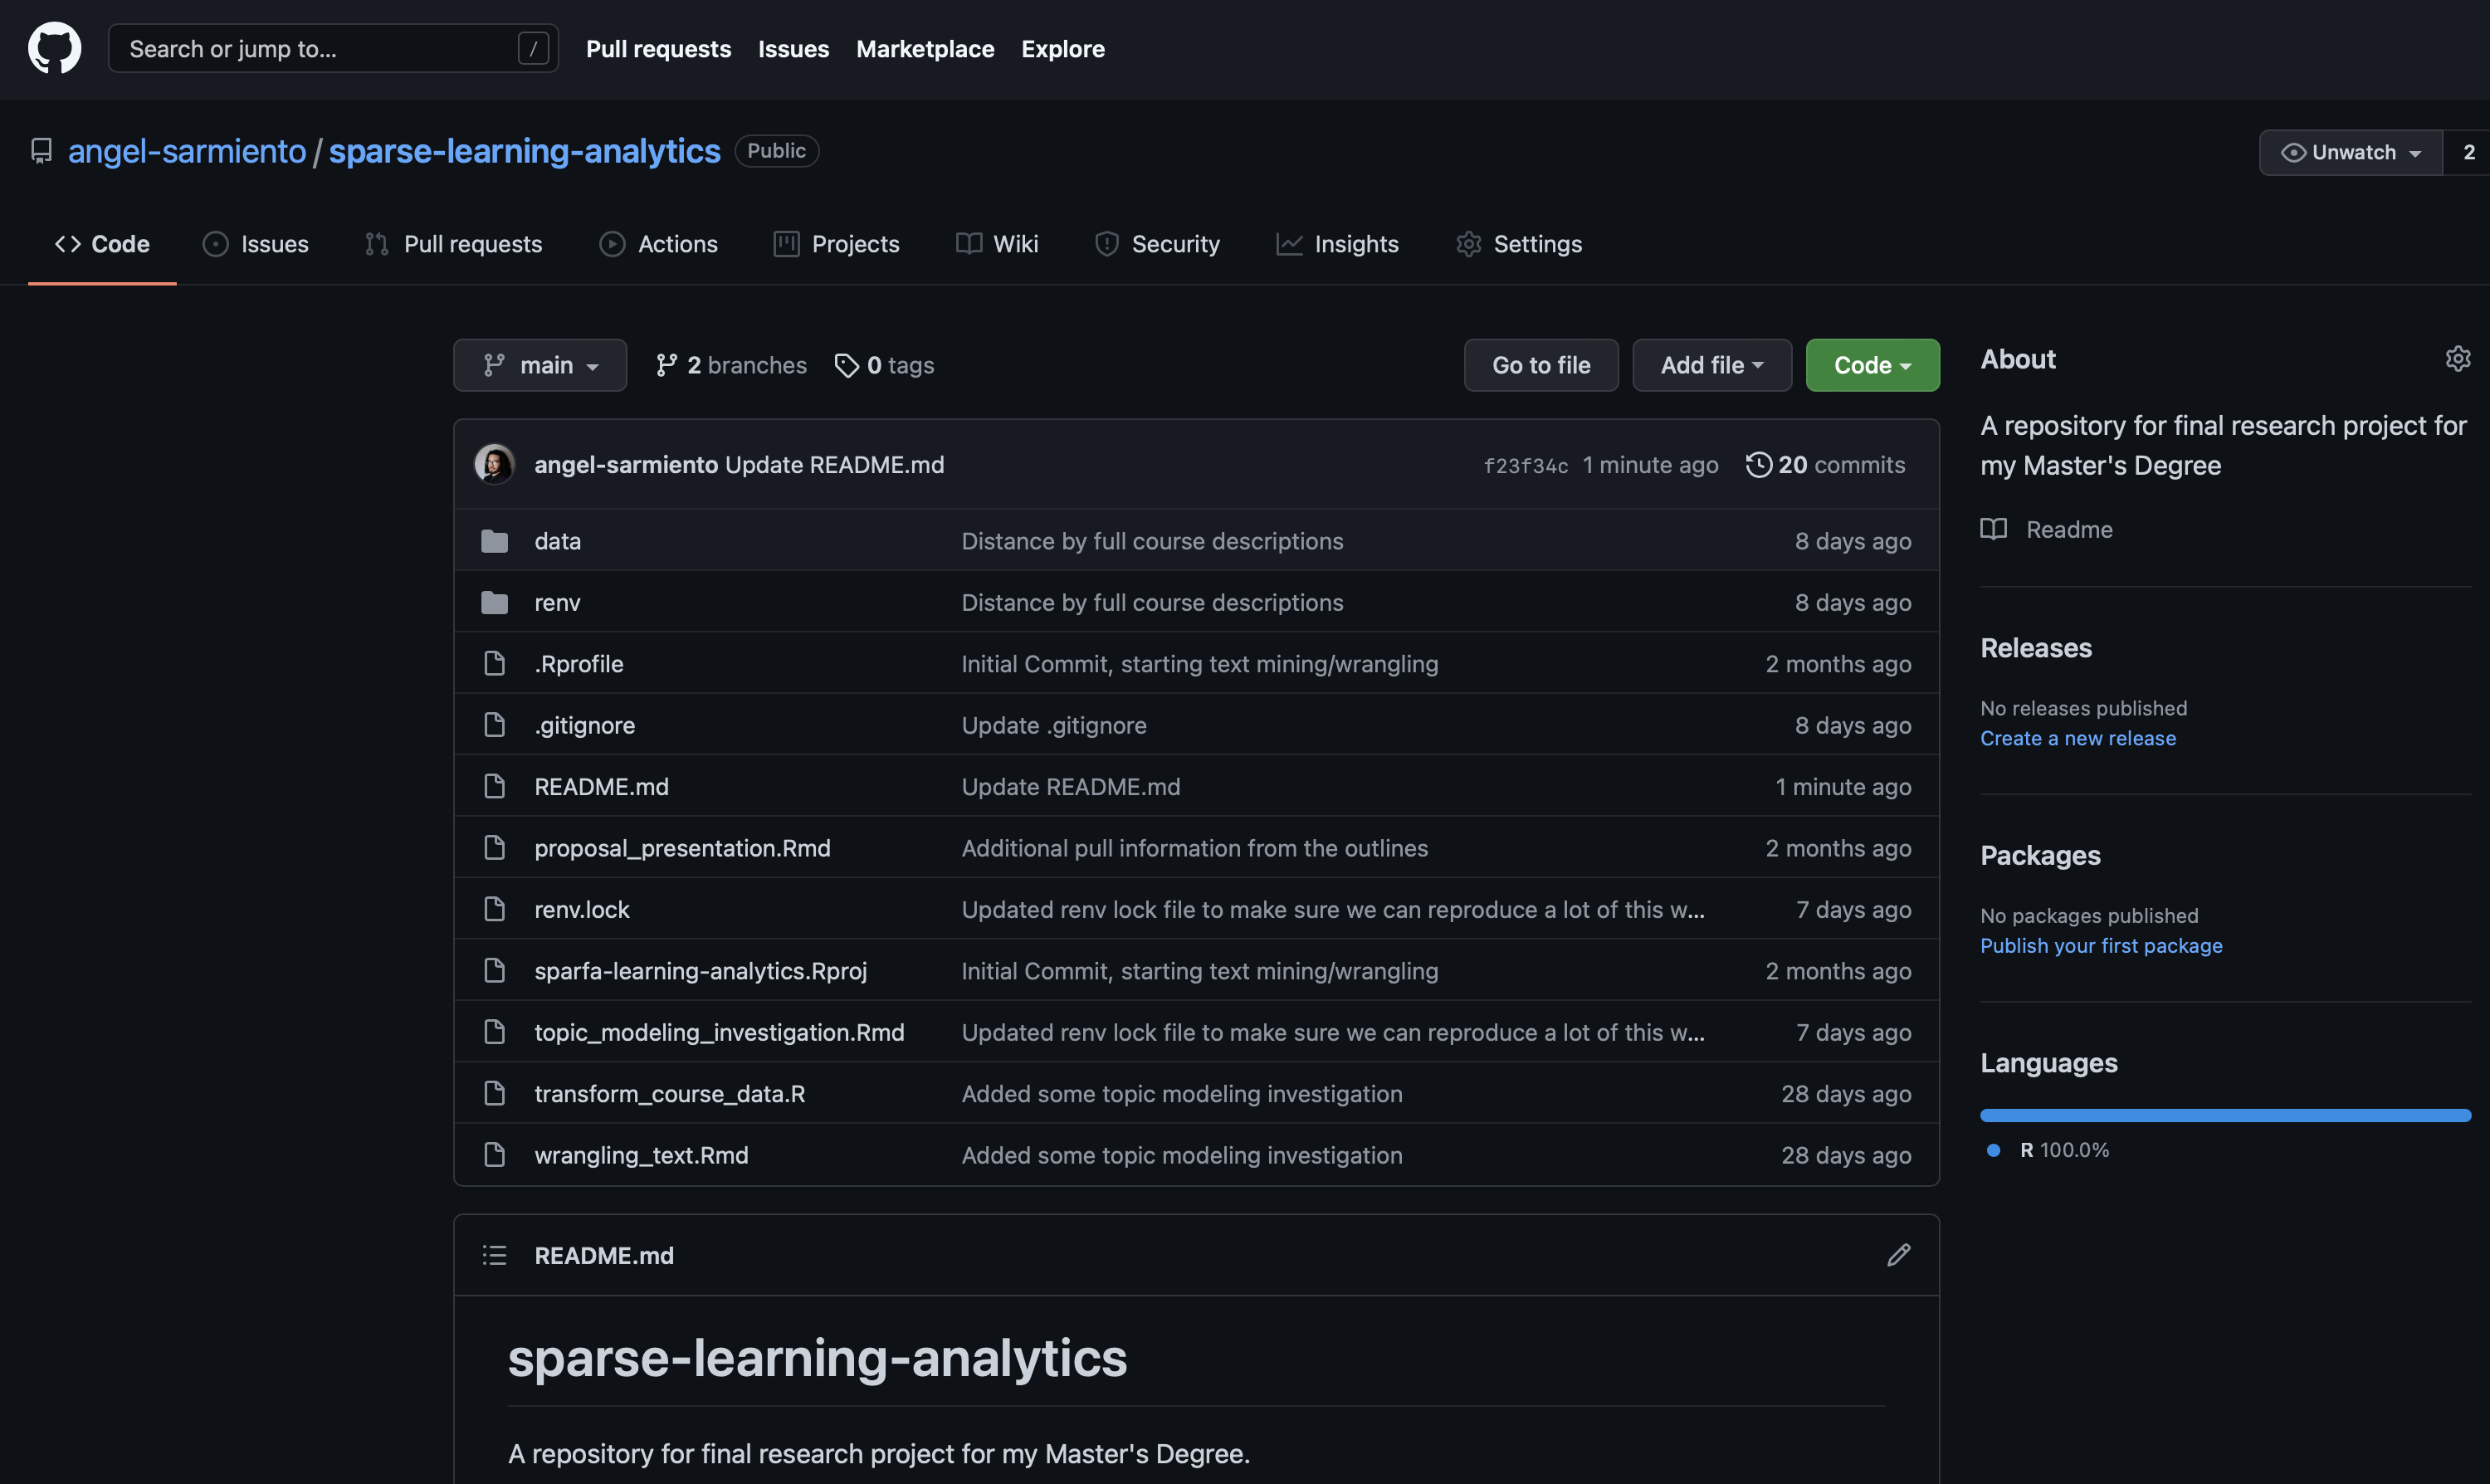
\includegraphics[width = \textwidth, height = 0.5\textheight]{images/repo.png}
\caption{Open-source GitHub repository}
\label{fig:repo}
\end{figure}


\subsection{Correspondence Analysis}
\label{ca} 

The project started with implementations of MCA on bigrams of the course outlines,  first cleaning the data using regular expressions \citep{regex} and custom functions.  The 4 latent dimensions produced from MCA were plotted to show some of the associations created.  Figure \ref{fig:mca_2} shows a biplot with the third and fourth latent dimensions


\begin{figure}[H]
\centering

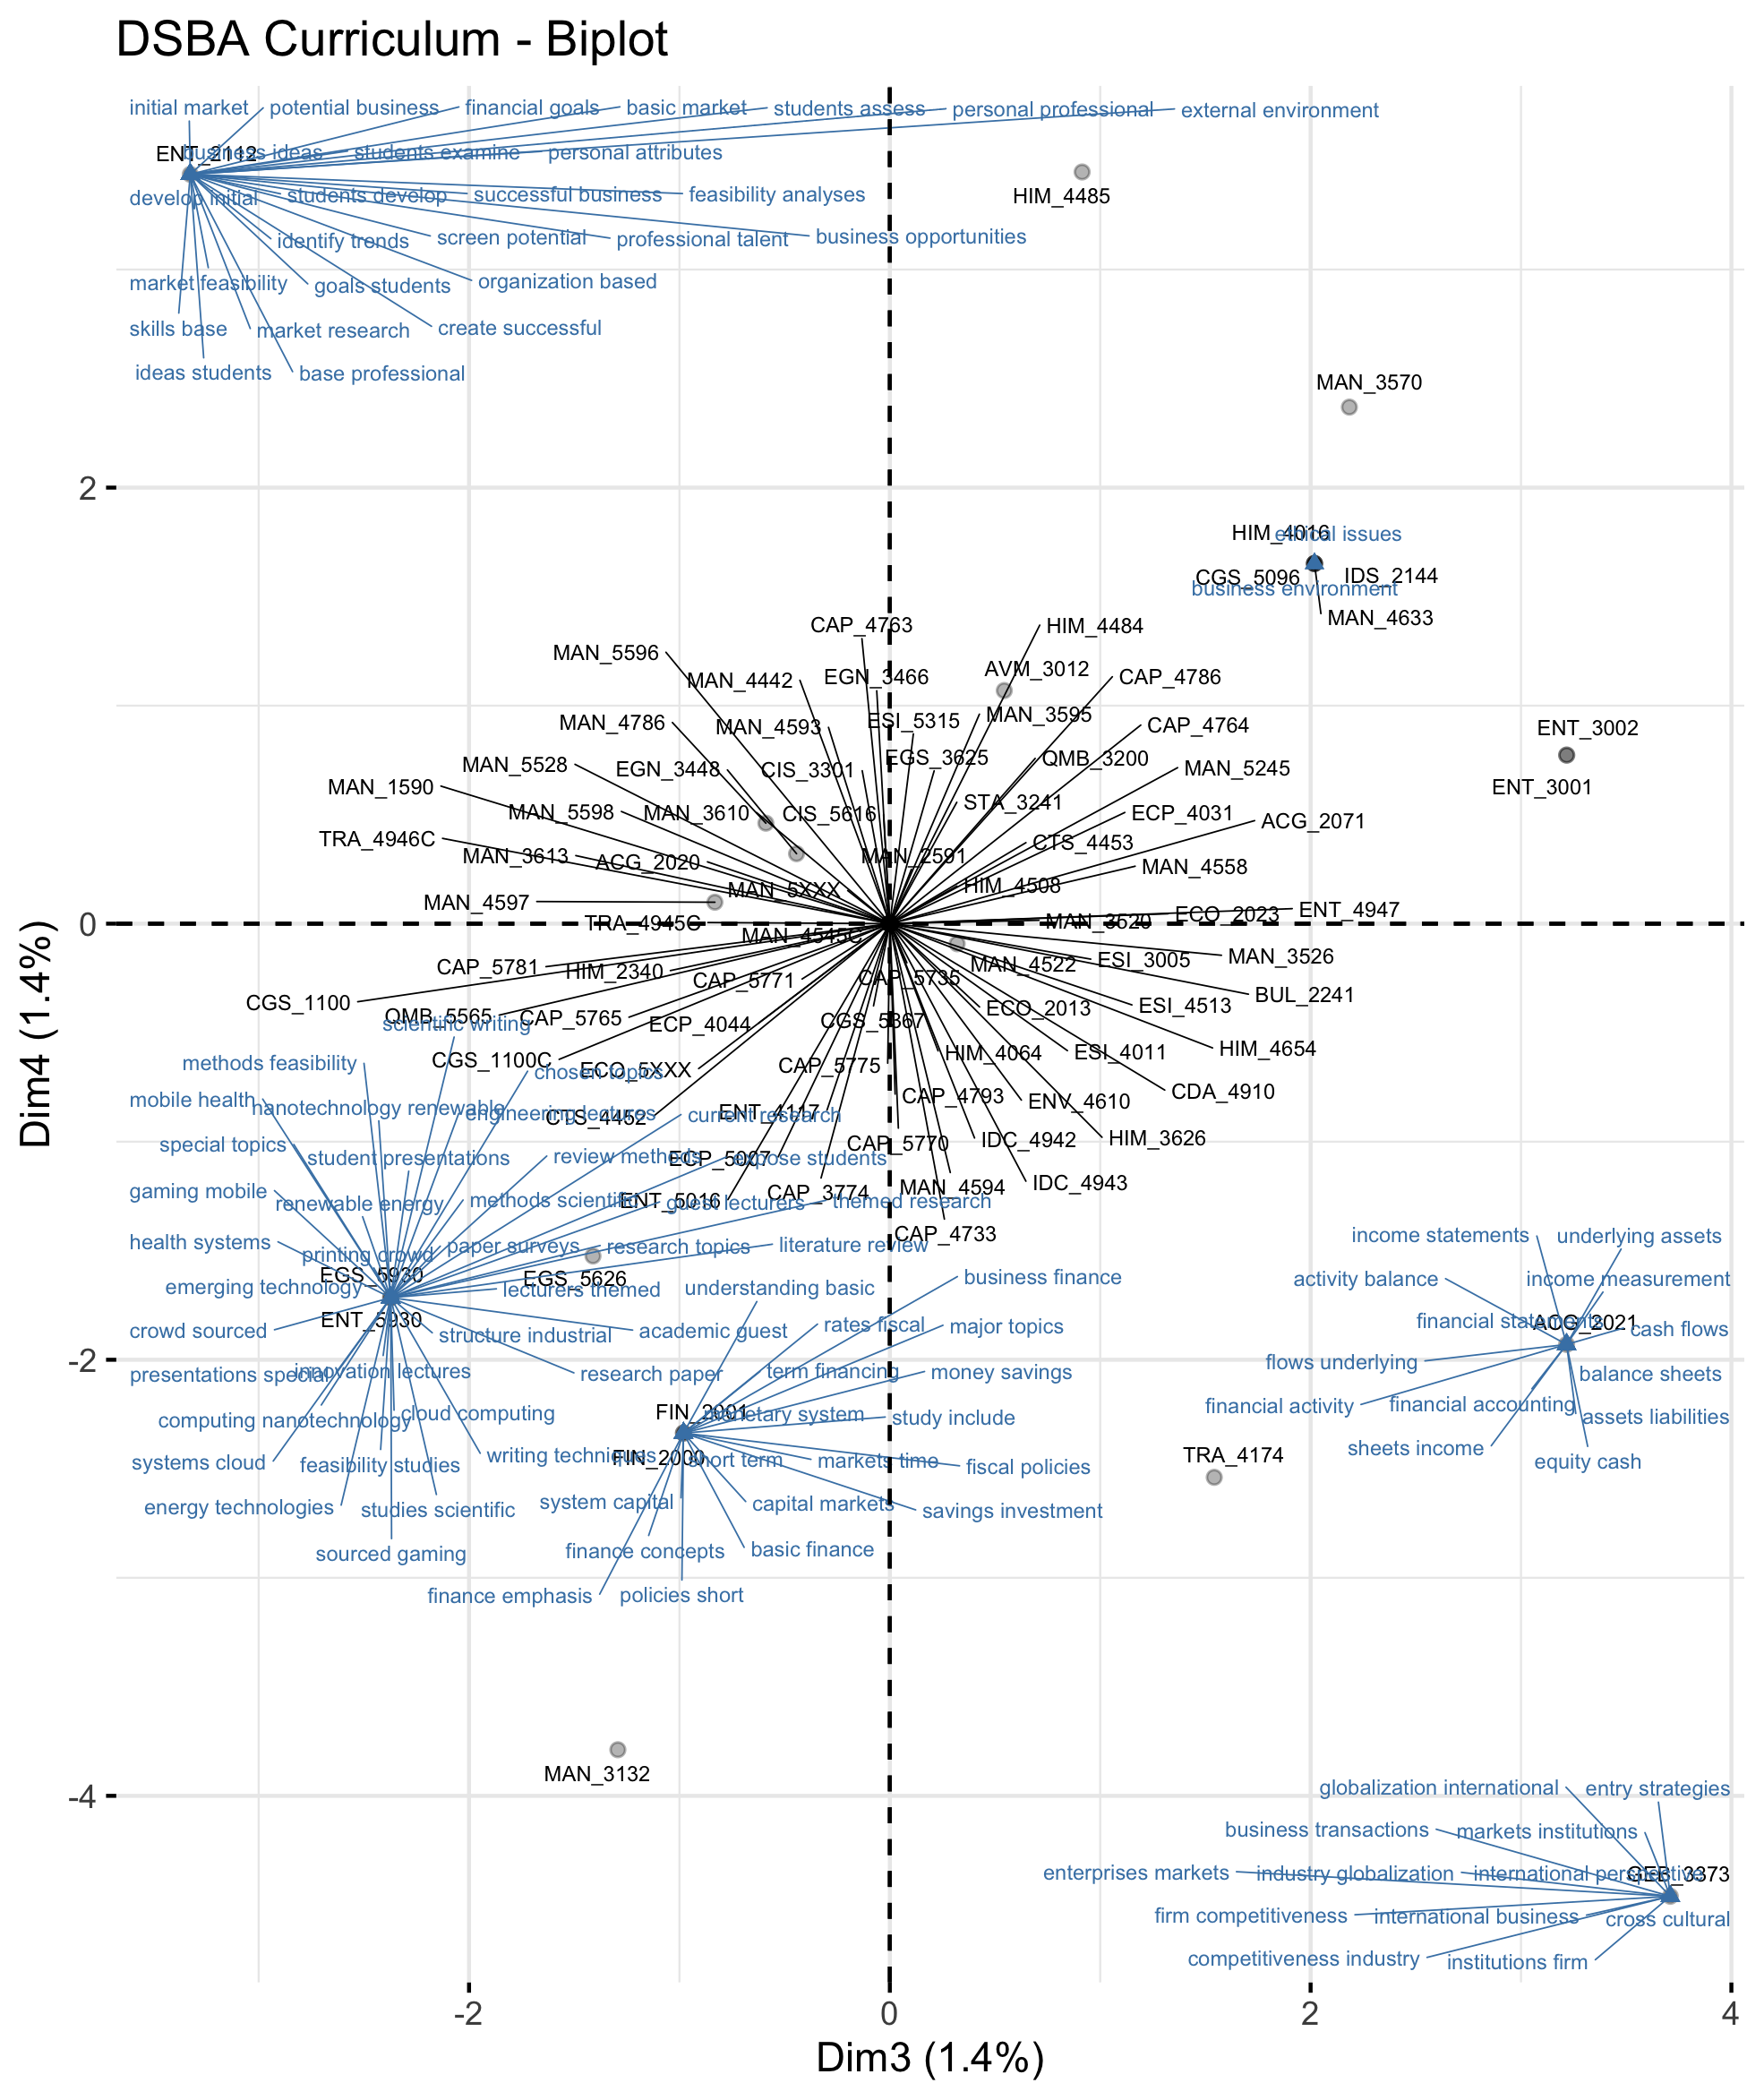
\includegraphics[width = 1\textwidth, height = .78\textheight]{images/mca_bp_2.png}
\caption{Biplot of the DSBA curriculum at FPU,  the top 100 topics and top 30 courses in terms of contribution to the proportion of variance are plotted.}
\label{fig:mca_2}
\end{figure}

Figure \ref{fig:mca_2} shows the potential groupings formed with this methodology.  In the central cluster of courses, a majority of the "MAN" courses occupy the second quadrant while the courses heavier in math and programming like statistical learning (STA 3241),  quantitative methods (QMB 3200), and others show up in the first quadrant.  The further from the center, the more "niche" the courses (typically business courses like ENT 2112 or ACG 2021) and course topics are.  This can potentially be used in the future as a backbone to the alignment of course work to corresponding concentrations in the future.

The plot above only shows a very small subset of the bigrams created from the course outlines since using all of them would not be legible.  Despite this,  some course-topic association can be seen.  For instance, two of the only financial courses in the curriculum, FIN 2001 and FIN 2000 occupy a small grouping in the third quadrant, unified by topics like "capital markets", "basic finance", and "savings investment". 

\subsection{Latent Dirichlet Allocation}

In developing this project, we wanted to see if well-defined course concentrations were evident from the results of Unsupervised learning techniques applied to the text data from the catalog using just the bigrams of the course descriptions.  To do this,  we started with similar data cleaning steps as before, except with the course descriptions used to fit a LDA \citep{lda_pap} topic model to identify the 5 different course concentrations in the DSBA curriculum. 

The five concentrations are as follows:   
\begin{itemize}
	\item{Logistics \& Supply Chain Management }
	\item{Intelligent Mobility}
	\item{Quantitative Economics and Econometrics}
	\item{Big Data Analytics}
	\item{Health Systems Engineering}

\end{itemize}

Our topic model was generated with Gibbs sampling for 500 iterations,  getting the document-term probabilities ($\beta$) and ordering in descending order by each topic. Figure \ref{fig:lda} shows the results.


\begin{figure}[H]
\centering

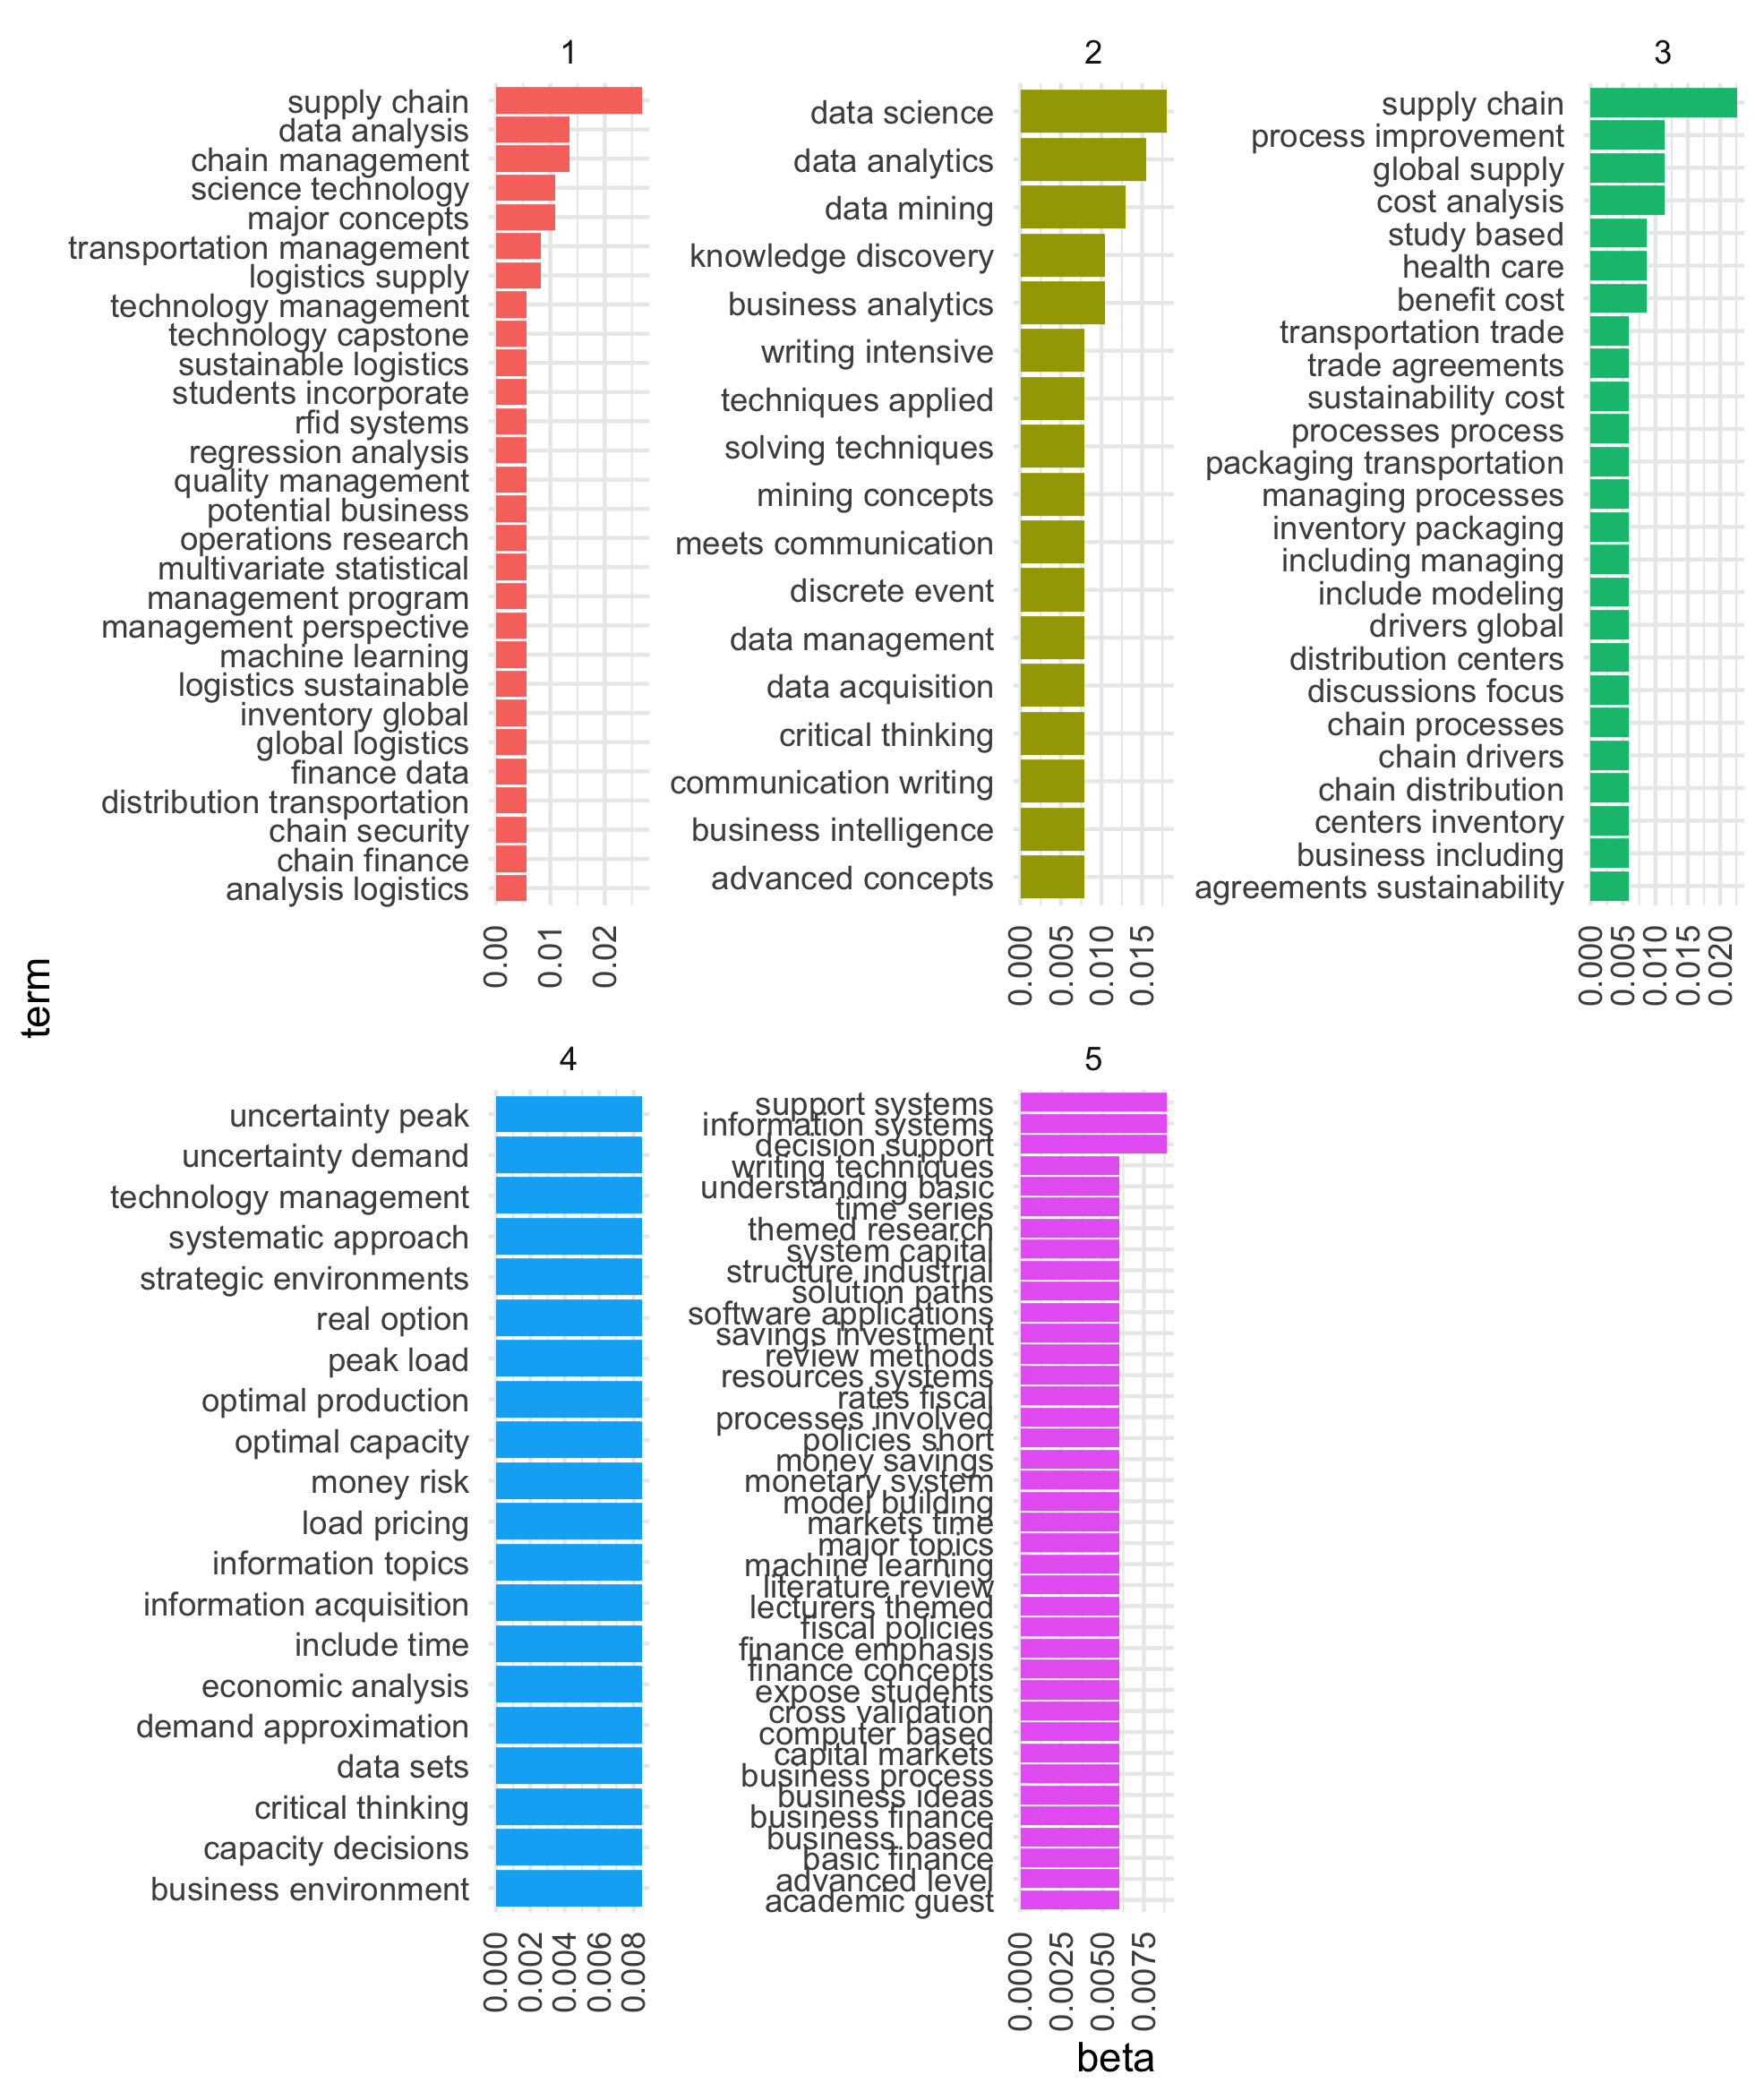
\includegraphics[width = .9\textwidth, height = .8\textheight]{images/lda.png}
\caption{LDA topic model splitting course topics into concentrations}
\label{fig:lda}
\end{figure}

From Figure \ref{fig:lda} above, it is feasible to see that topics 1 and 3 could be in Logistics and Supply Chain Management, topic 4 is most likely Quantitative Economics and Econometrics while Big Data Analytics could be topic 2. The segmentation across concentrations is not perfect however, where topics like "machine learning" and "regression analysis" show large betas in topic 1, while not being shown in other topics like topics 2 and 4 where one might think to find them very proliferate. This seems to be a limitation on the course descriptions and how they differ in size from course to course.  

The beta values represent the \textit{topic-word density}, meaning that higher betas represent a higher number of words that make up a topic.  A lower beta value places more weight on fewer, more "dominant" words in the corpus.  Conversely,  higher betas for topics indicate that the topic is assumed to made of up \textit{most} of the words in the entire corpus.  For topics 1 and 2 in Figure \ref{fig:lda}, we see that "supply chain" has the highest beta value. This implies that this bigram appears very often in the overall corpus of bigrams in the entire dataset and that supply chain is highly likely to be in one or both of those topics.  Topic 5 is filled with bigrams with very small beta values in comparison,  implying that something like "capital markets" does not appear very often in the overall corpus with a beta value of around $0.0055$,  but groups with other less prevalent words in defining this topic.  Since topic 5 relies on a set of bigrams that do not appear as much in the overall dataset, it possibly implies that these bigrams or concepts are niche relative to the entire catalog of concepts.


\subsection{Multidimensional Scaling}

In order to develop association graphs, we created multiple distance matrices using a variety of different distance metrics.  Some of the distance metrics we used are: 
\begin{itemize}
\item Euclidean distance  
$$\sqrt{\Sigma_{i = 1}^{k}(x_i - y_i)^2}$$
where $x_i$ and $y_i$ are two corresponding documents (course descriptions or outlines) split into vectors of bigrams or vectors containing the full descriptions.
\item Cosine similarity
$$ \cos (\theta) = \frac{A \cdot B}{|| A || || B||}$$
where $\theta$ is the angle between two objects, denoting the similarity.  $||A||$ and $||B||$ are the Euclidean Norm or length of two vectors (in this case, course descriptions or course outline vectors). $A \cdot B$ is the dot product  between two course descriptions or course outlines. 
\item Jaccard similarity  
$$\frac{A \cap B}{A \cup B}$$
where A and B are course descriptions or course outlines in vector form, and we are calculating the intersection divided by the union between the two vectors.
\item Burrow's Delta  \citep{burrow}
$$\Delta_B = \Sigma_{i = 1}^n | z_i(D_1) - z_i(D_2)|$$
where $z_i(D) = (f_i(D) - \mu_i/\sigma_i)$ or the standardized z-score for document $D$ and word $i$.  Word frequencies then follow the distribution described by Zipf's law \citep{zipf2013psycho}. 

\end{itemize} 

We experimented in plotting relative distances of courses based on the pairwise distance between all of the courses' full course descriptions (not bigrams).  We used whole course descriptions to combat the potential weaknesses in the n-gram approach not including the entire context of the descriptions.   Figure \ref{fig:tile} shows a comparison between Jaccard and Cosine distances, the two metrics that resulted in better performance in terms of interpretability,  for the text data considered in this study. Both of these metrics show mostly defined groupings and display interesting insights. The lighter color of the line connecting two courses, the further the distance between them.


\begin{figure}[H]
\centering
\begin{subfigure}{.5\textwidth}
  \centering
  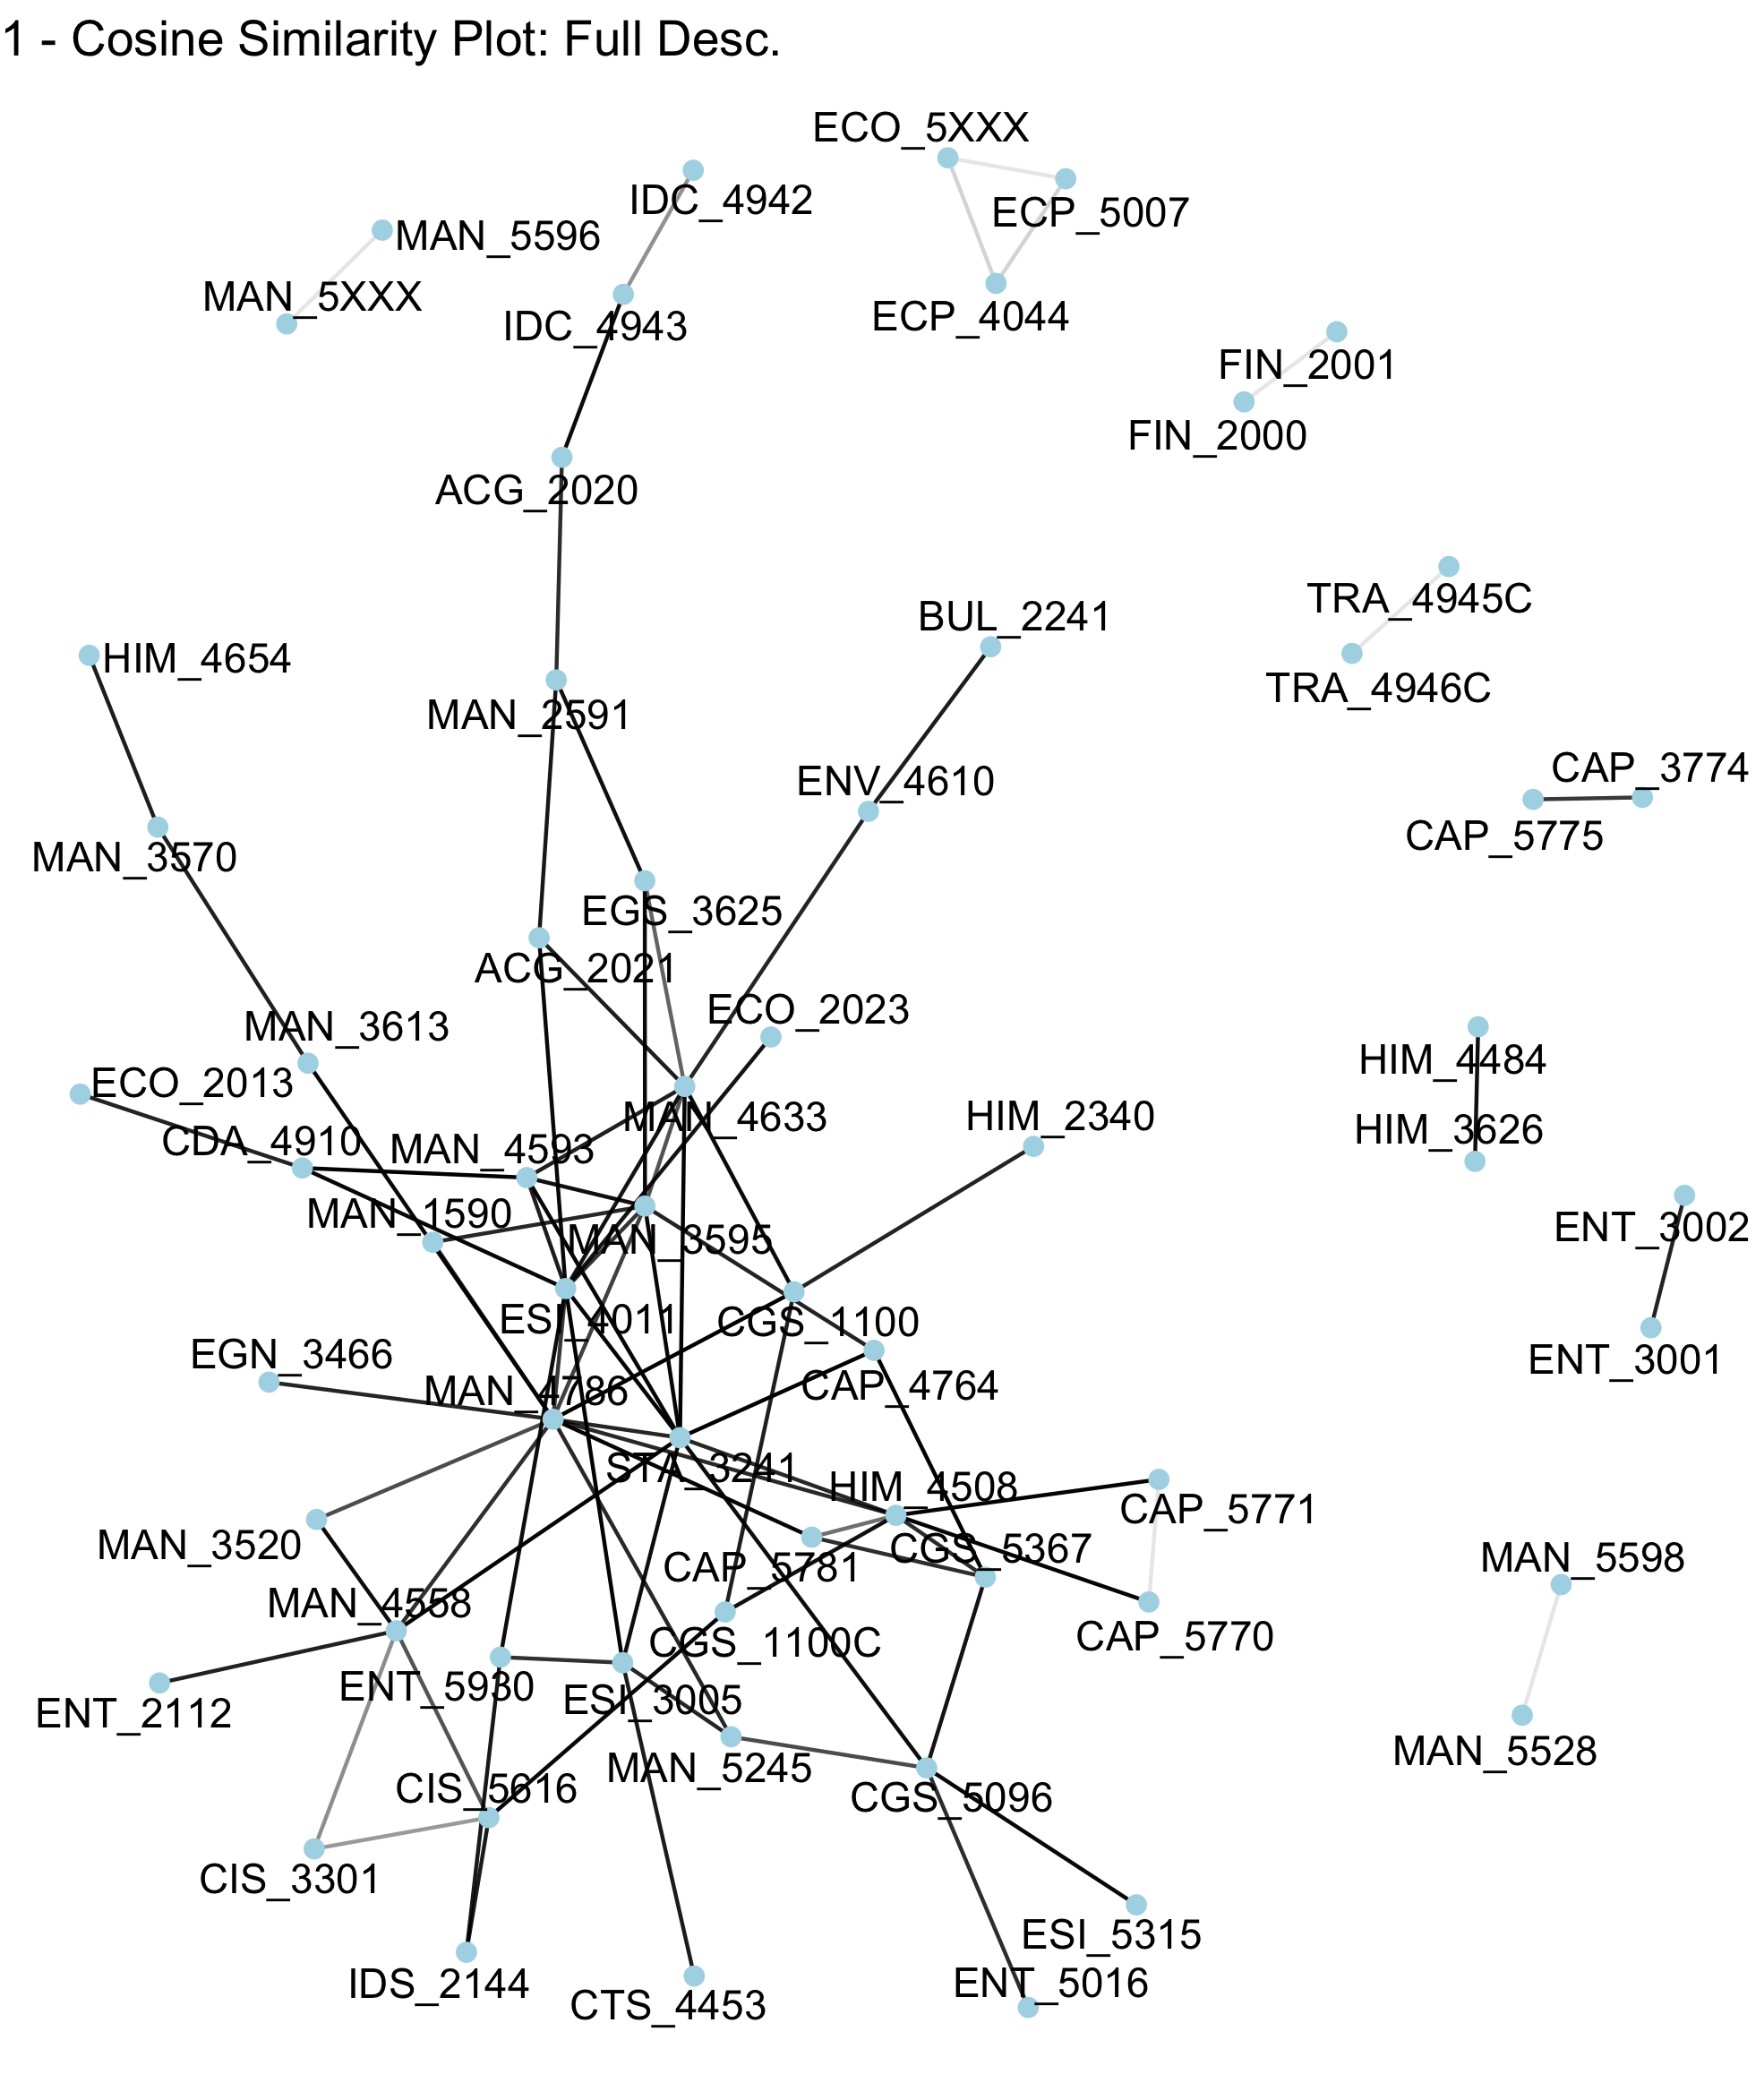
\includegraphics[width=1\linewidth]{images/cos.png}
  \caption{Cosine Distance}
  \label{fig:cos}
\end{subfigure}%
\begin{subfigure}{.5\textwidth}
  \centering
  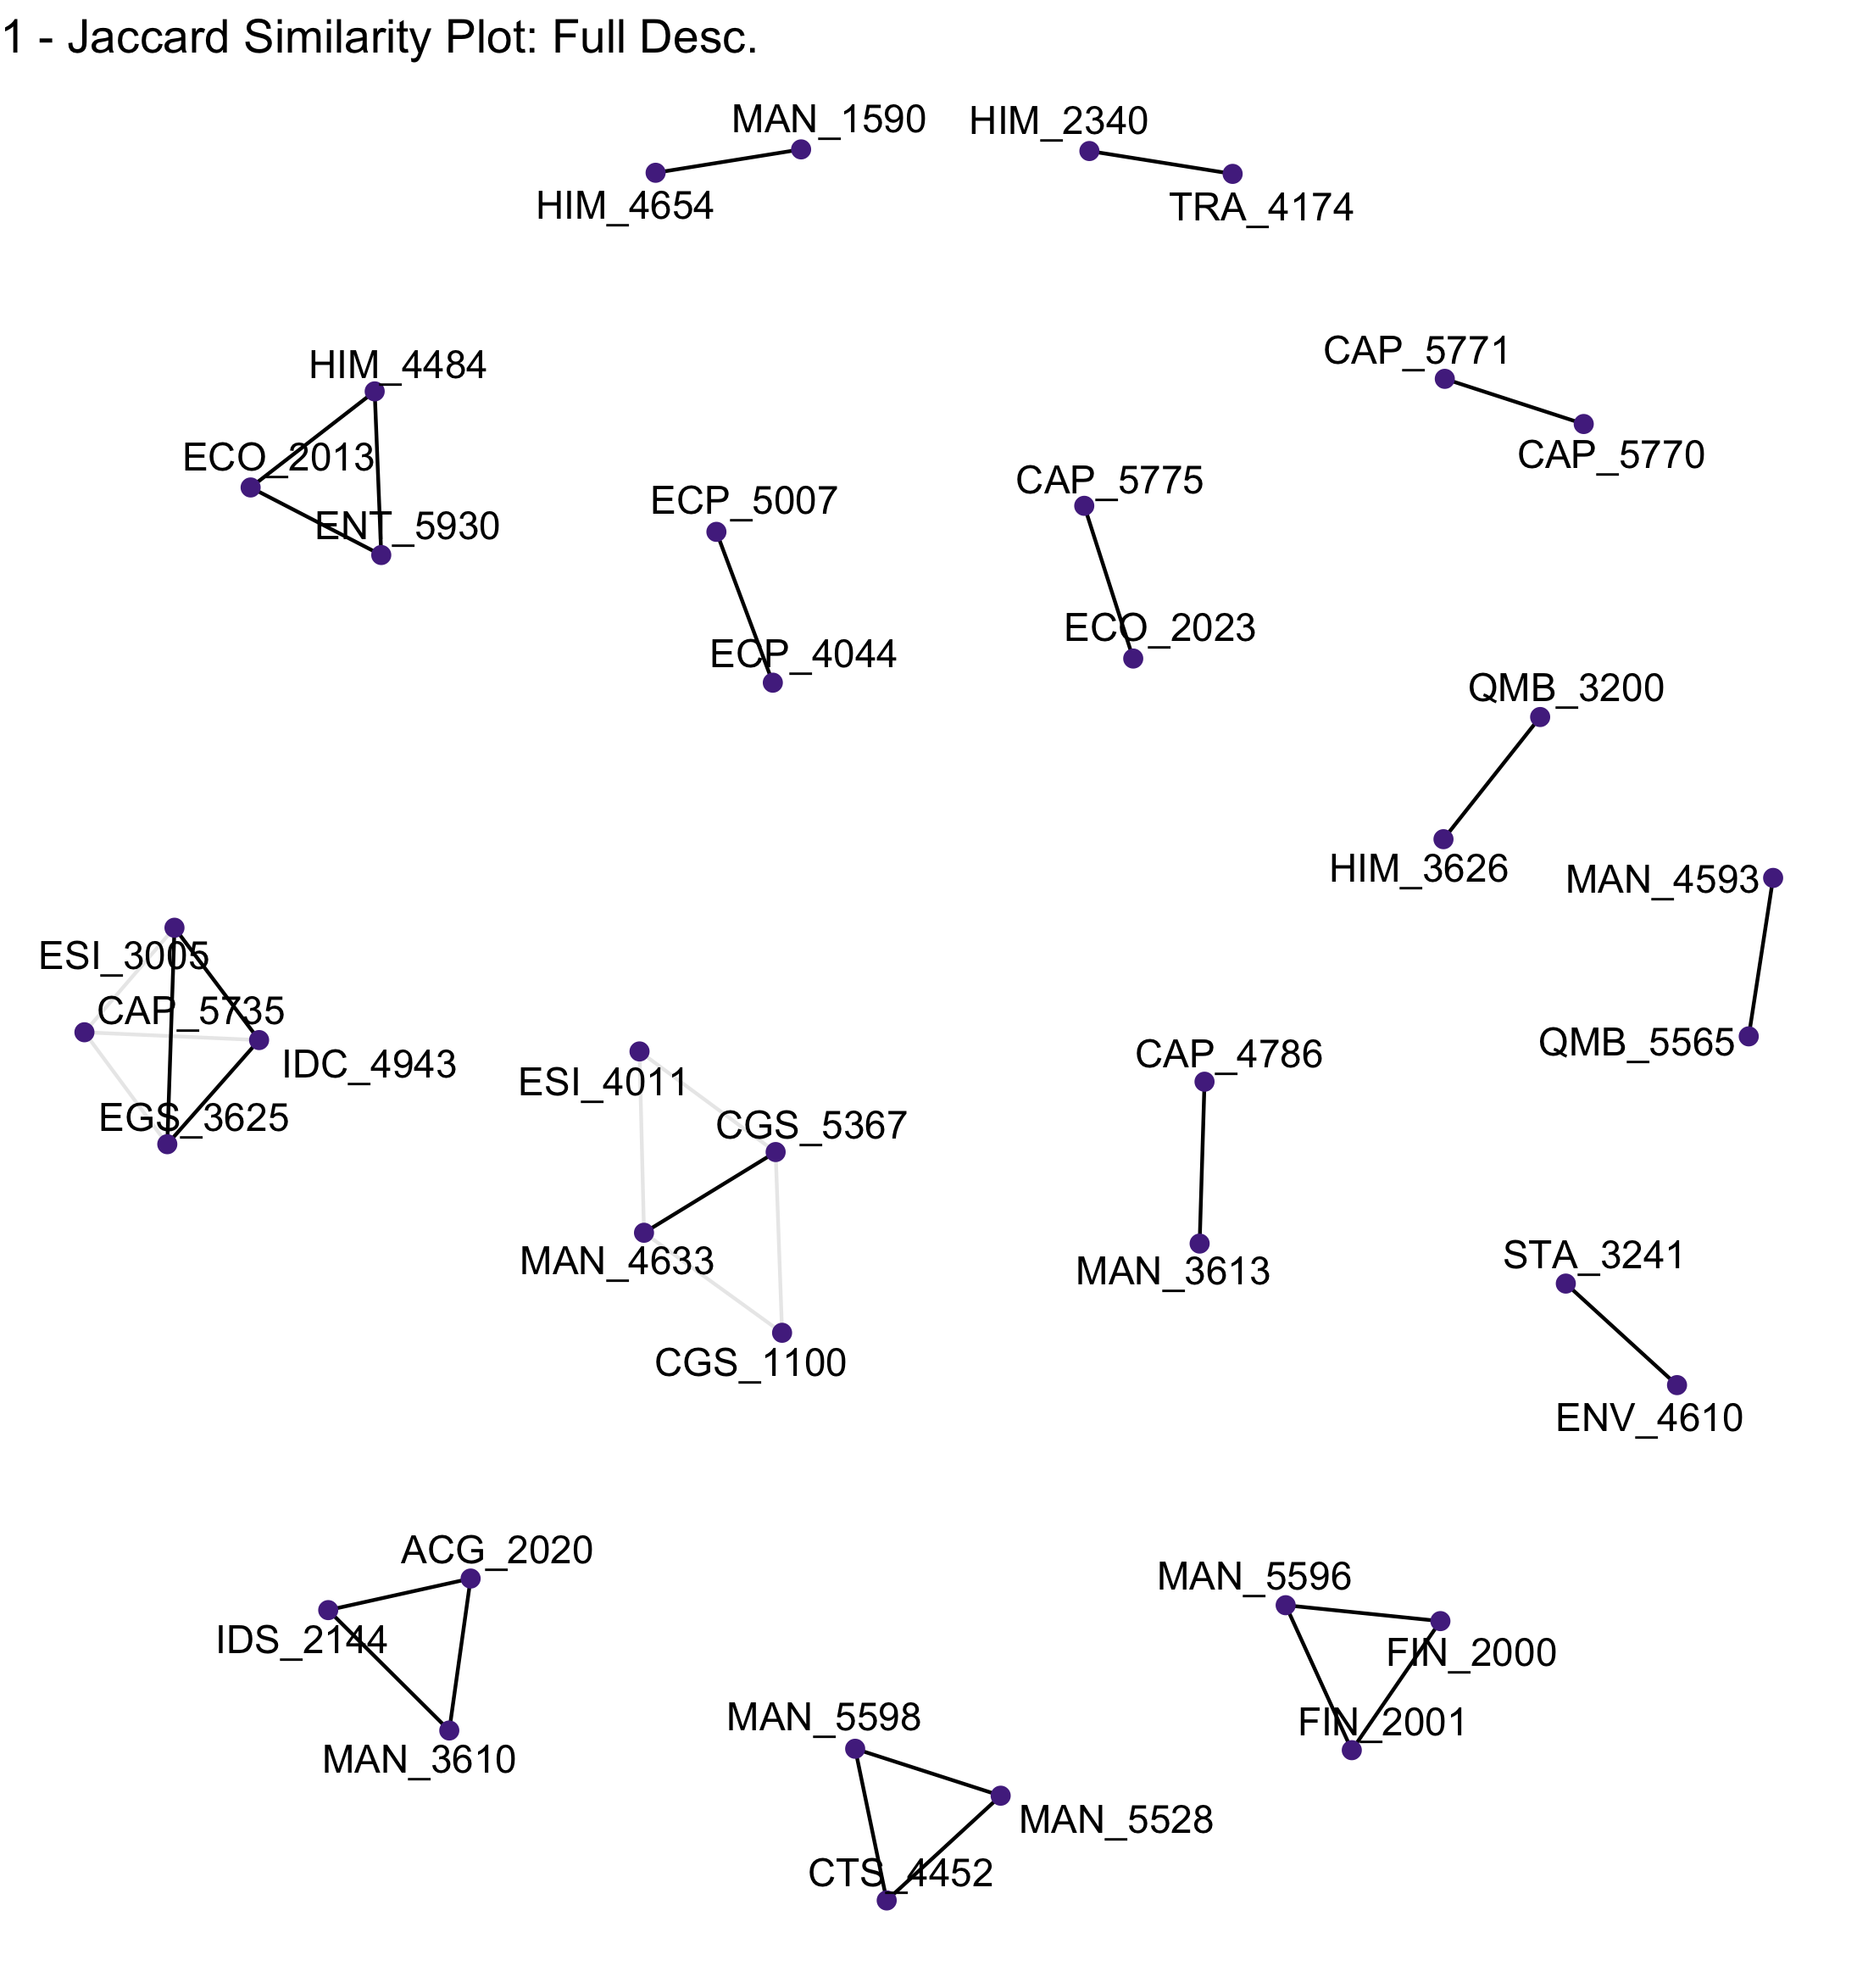
\includegraphics[width=1\linewidth]{images/jac.png}
  \caption{Jaccard Distance}
  \label{fig:jac}
\end{subfigure}
\caption{Comparison between the two best distance metrics}
\label{fig:tile}
\end{figure}

One common trait that became prevalent was the existence of common strings at the end of certain courses.  A majority of the courses that meet a writing requirement have the same course descriptions detailing:

 \textit{"This course meets communication/writing-intensive requirements (W)"} 
 
This seems to cause certain courses to be grouped together (have a smaller distance between them).  This is relatively consistent across the catalog and can be seen at the bottom of the plot on Figure \ref{fig:cos} with courses like ECO 2013. 

These distance matrices can then be used to apply a method like MDS to separate courses into clusters in latent spaces similar to section \ref{ca}. Ideally, we should see relatively defined groupings where we can make inferences on the placement of the courses within those groupings within the latent dimensions.  Figure \ref{fig:tile2} shows the same distance metrics in Figure \ref{fig:tile} used in our MDS implementation.

\begin{figure}[H]
\centering
\begin{subfigure}{.5\textwidth}
  \centering
  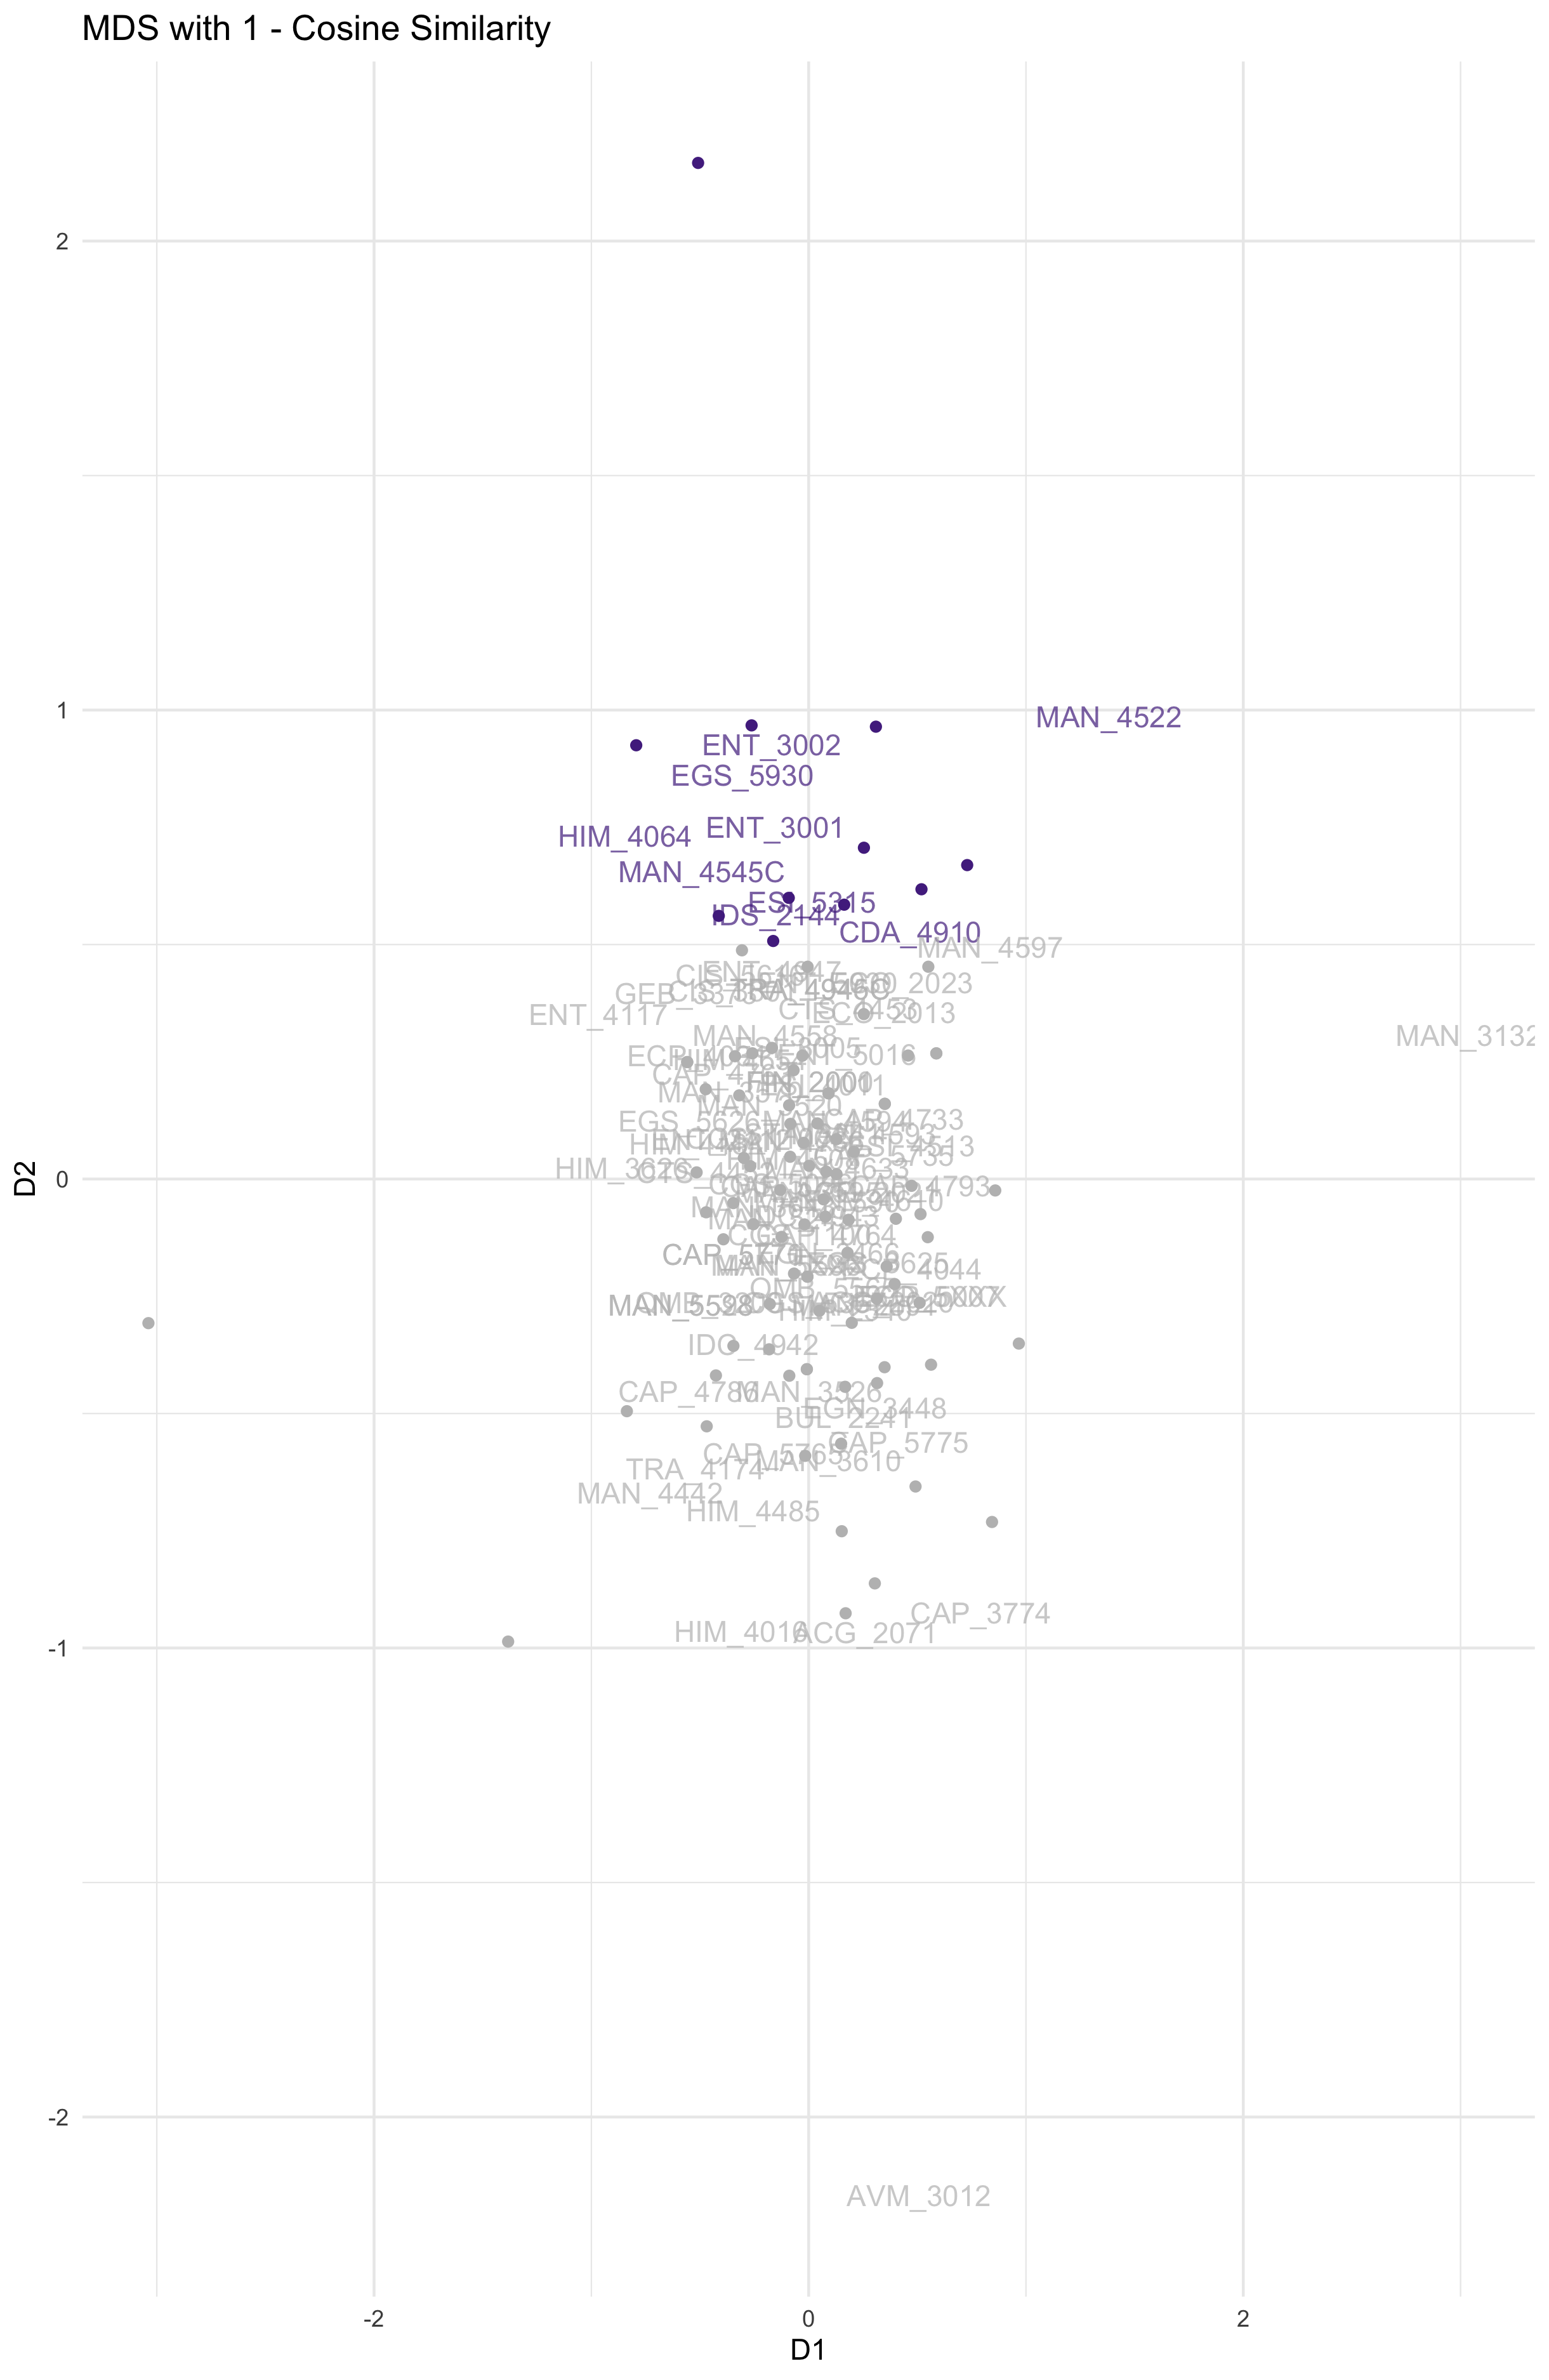
\includegraphics[width=1\linewidth]{images/cos_mds.png}
  \caption{Cosine Distance}
  \label{fig:cmds}
\end{subfigure}%
\begin{subfigure}{.5\textwidth}
  \centering
  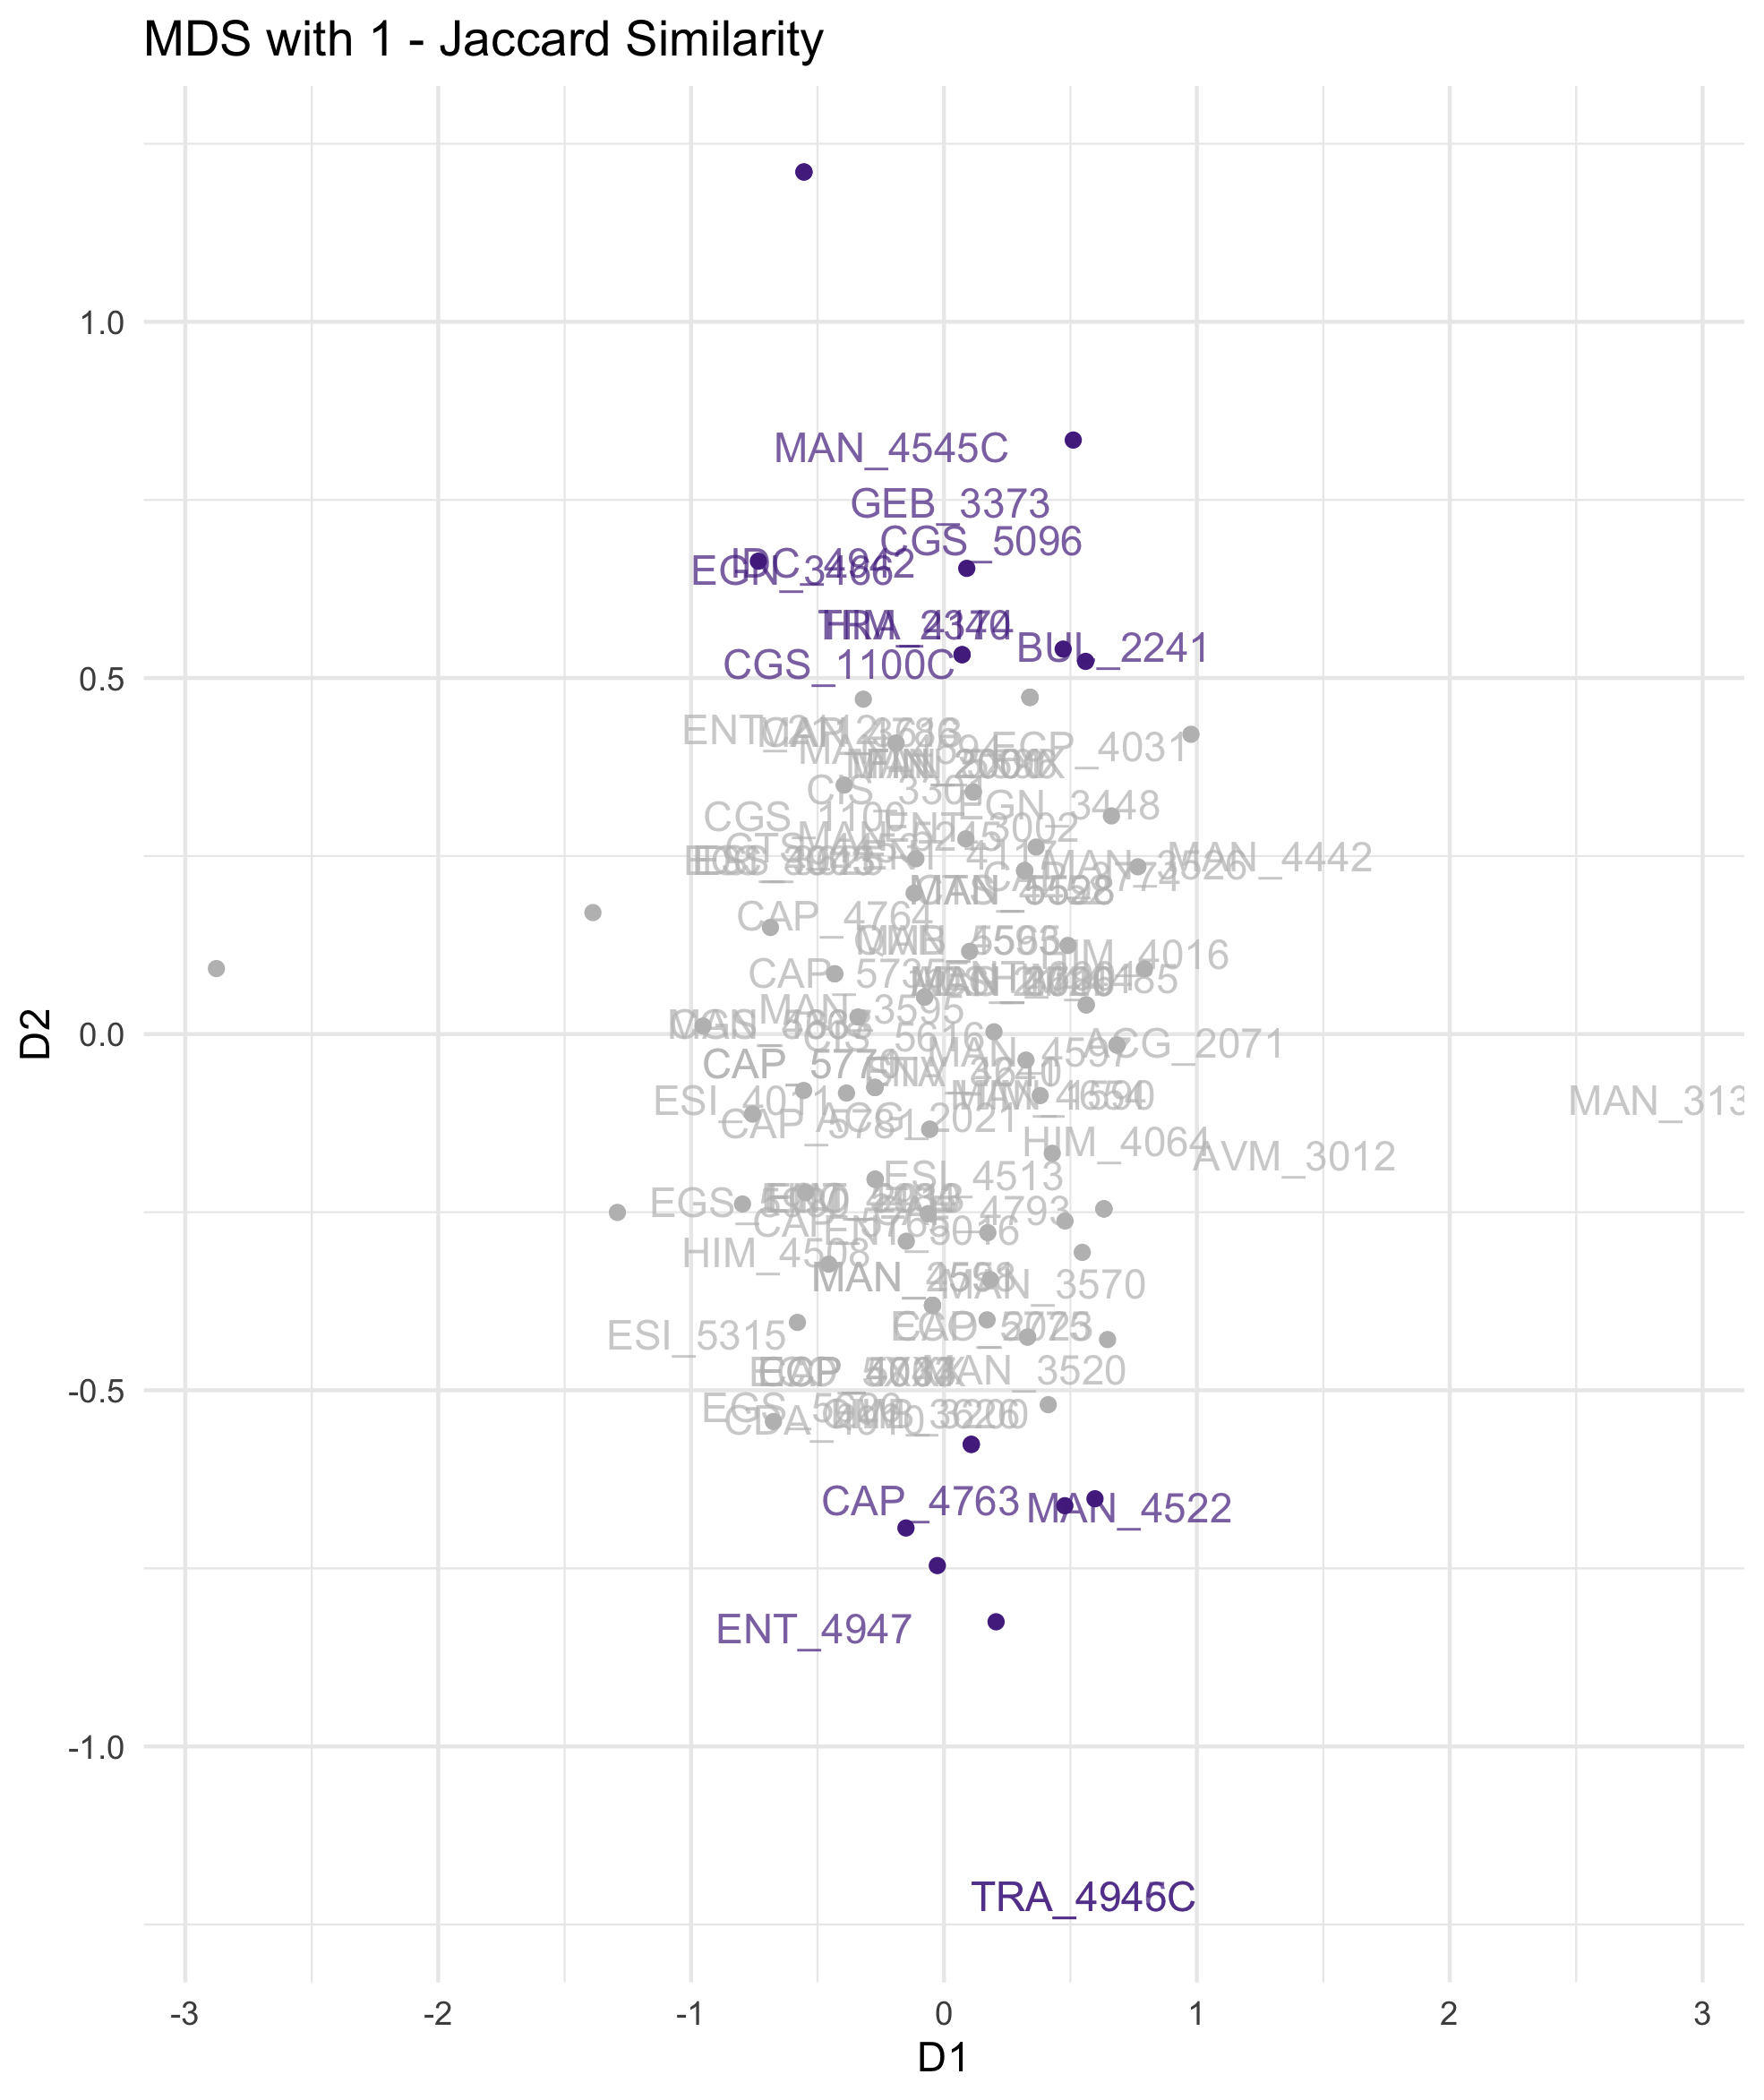
\includegraphics[width=1\linewidth]{images/jac_mds.png}
  \caption{Jaccard Distance}
  \label{fig:jmds}
\end{subfigure}
\caption{Comparison between MDS with Cosine distance and Jaccard distance}
\label{fig:tile2}
\end{figure}

From these plots we see that a grouping separation does not occur.  A majority of the courses group together in the middle within forming those defined groupings that one might want to see. A potential reason for this may be the choice of distance metrics. in the future, other distance metrics might prove better for providing the segmentation necessary to differentiate the courses using this full course description approach.  Another potential reason could be the size of q-grams used to compute the distances for each of the course descriptions: it is possible that different sized substrings might yield better results when computing the distance matrices. Increasing the size of the q-grams could potentially give the MDS dimensions more "context" from the larger substrings used to compute distances for MDS. 


%\section{Project Schedule}

%\begin{figure}[H]
%\centering

%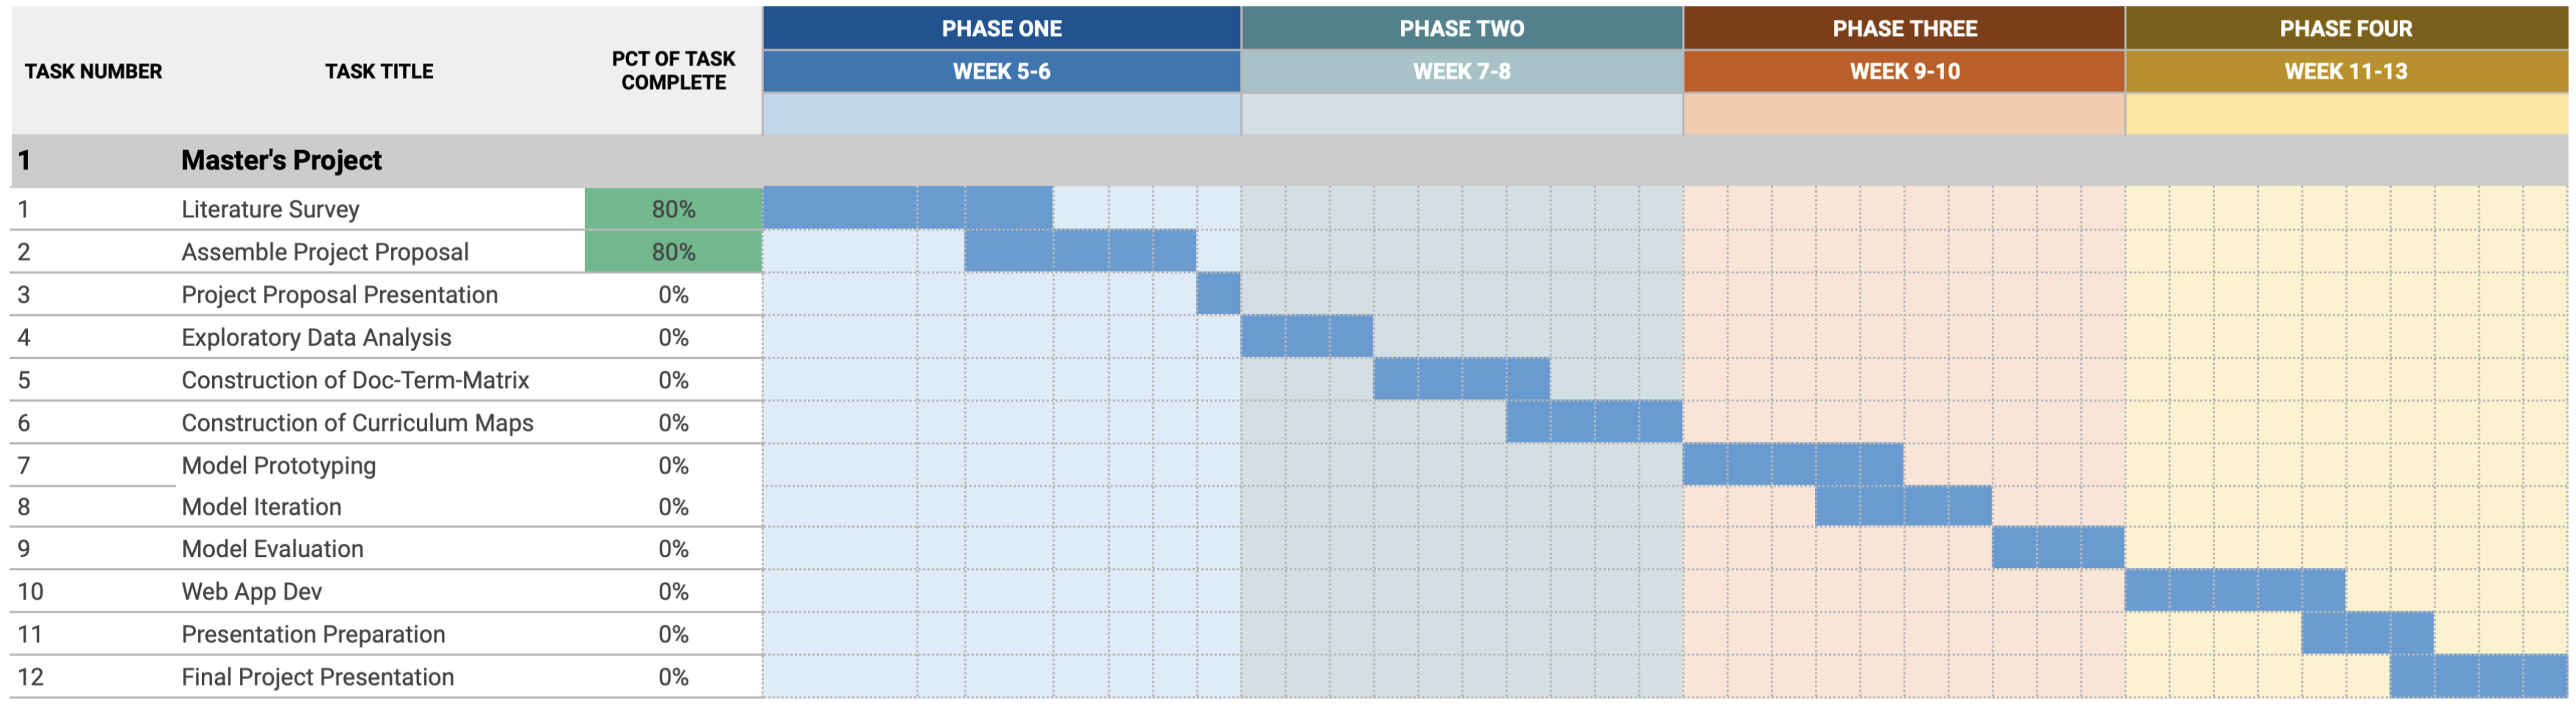
\includegraphics[width = \textwidth]{../images/schedule.png}
%\caption{Project Roadmap/ Gannt Chart}
%\label{fig:diagram}
%\end{figure}

\subsection{CS Plans of Study}

We can see how these models apply to the Computer Science plan of study as well. Figure \ref{fig:lda_cs} shows the LDA topic 
model and its ability to segment topics detected in the course outline bigrams into the 6 different concentrations present in CS (versus 5 concentrations in DSBA as we saw before). 
The concentrations for the CS plan of study are: 

\begin{itemize}
  \item Advanced Topics  
  \item Game Development \& Simulation  
  \item Information Assurance \& Cyber Security  
  \item Software Engineering   
  \item Autonomous Systems  
  \item Big Data Analytics  
\end{itemize}

\begin{figure}[H]
  \centering
  
  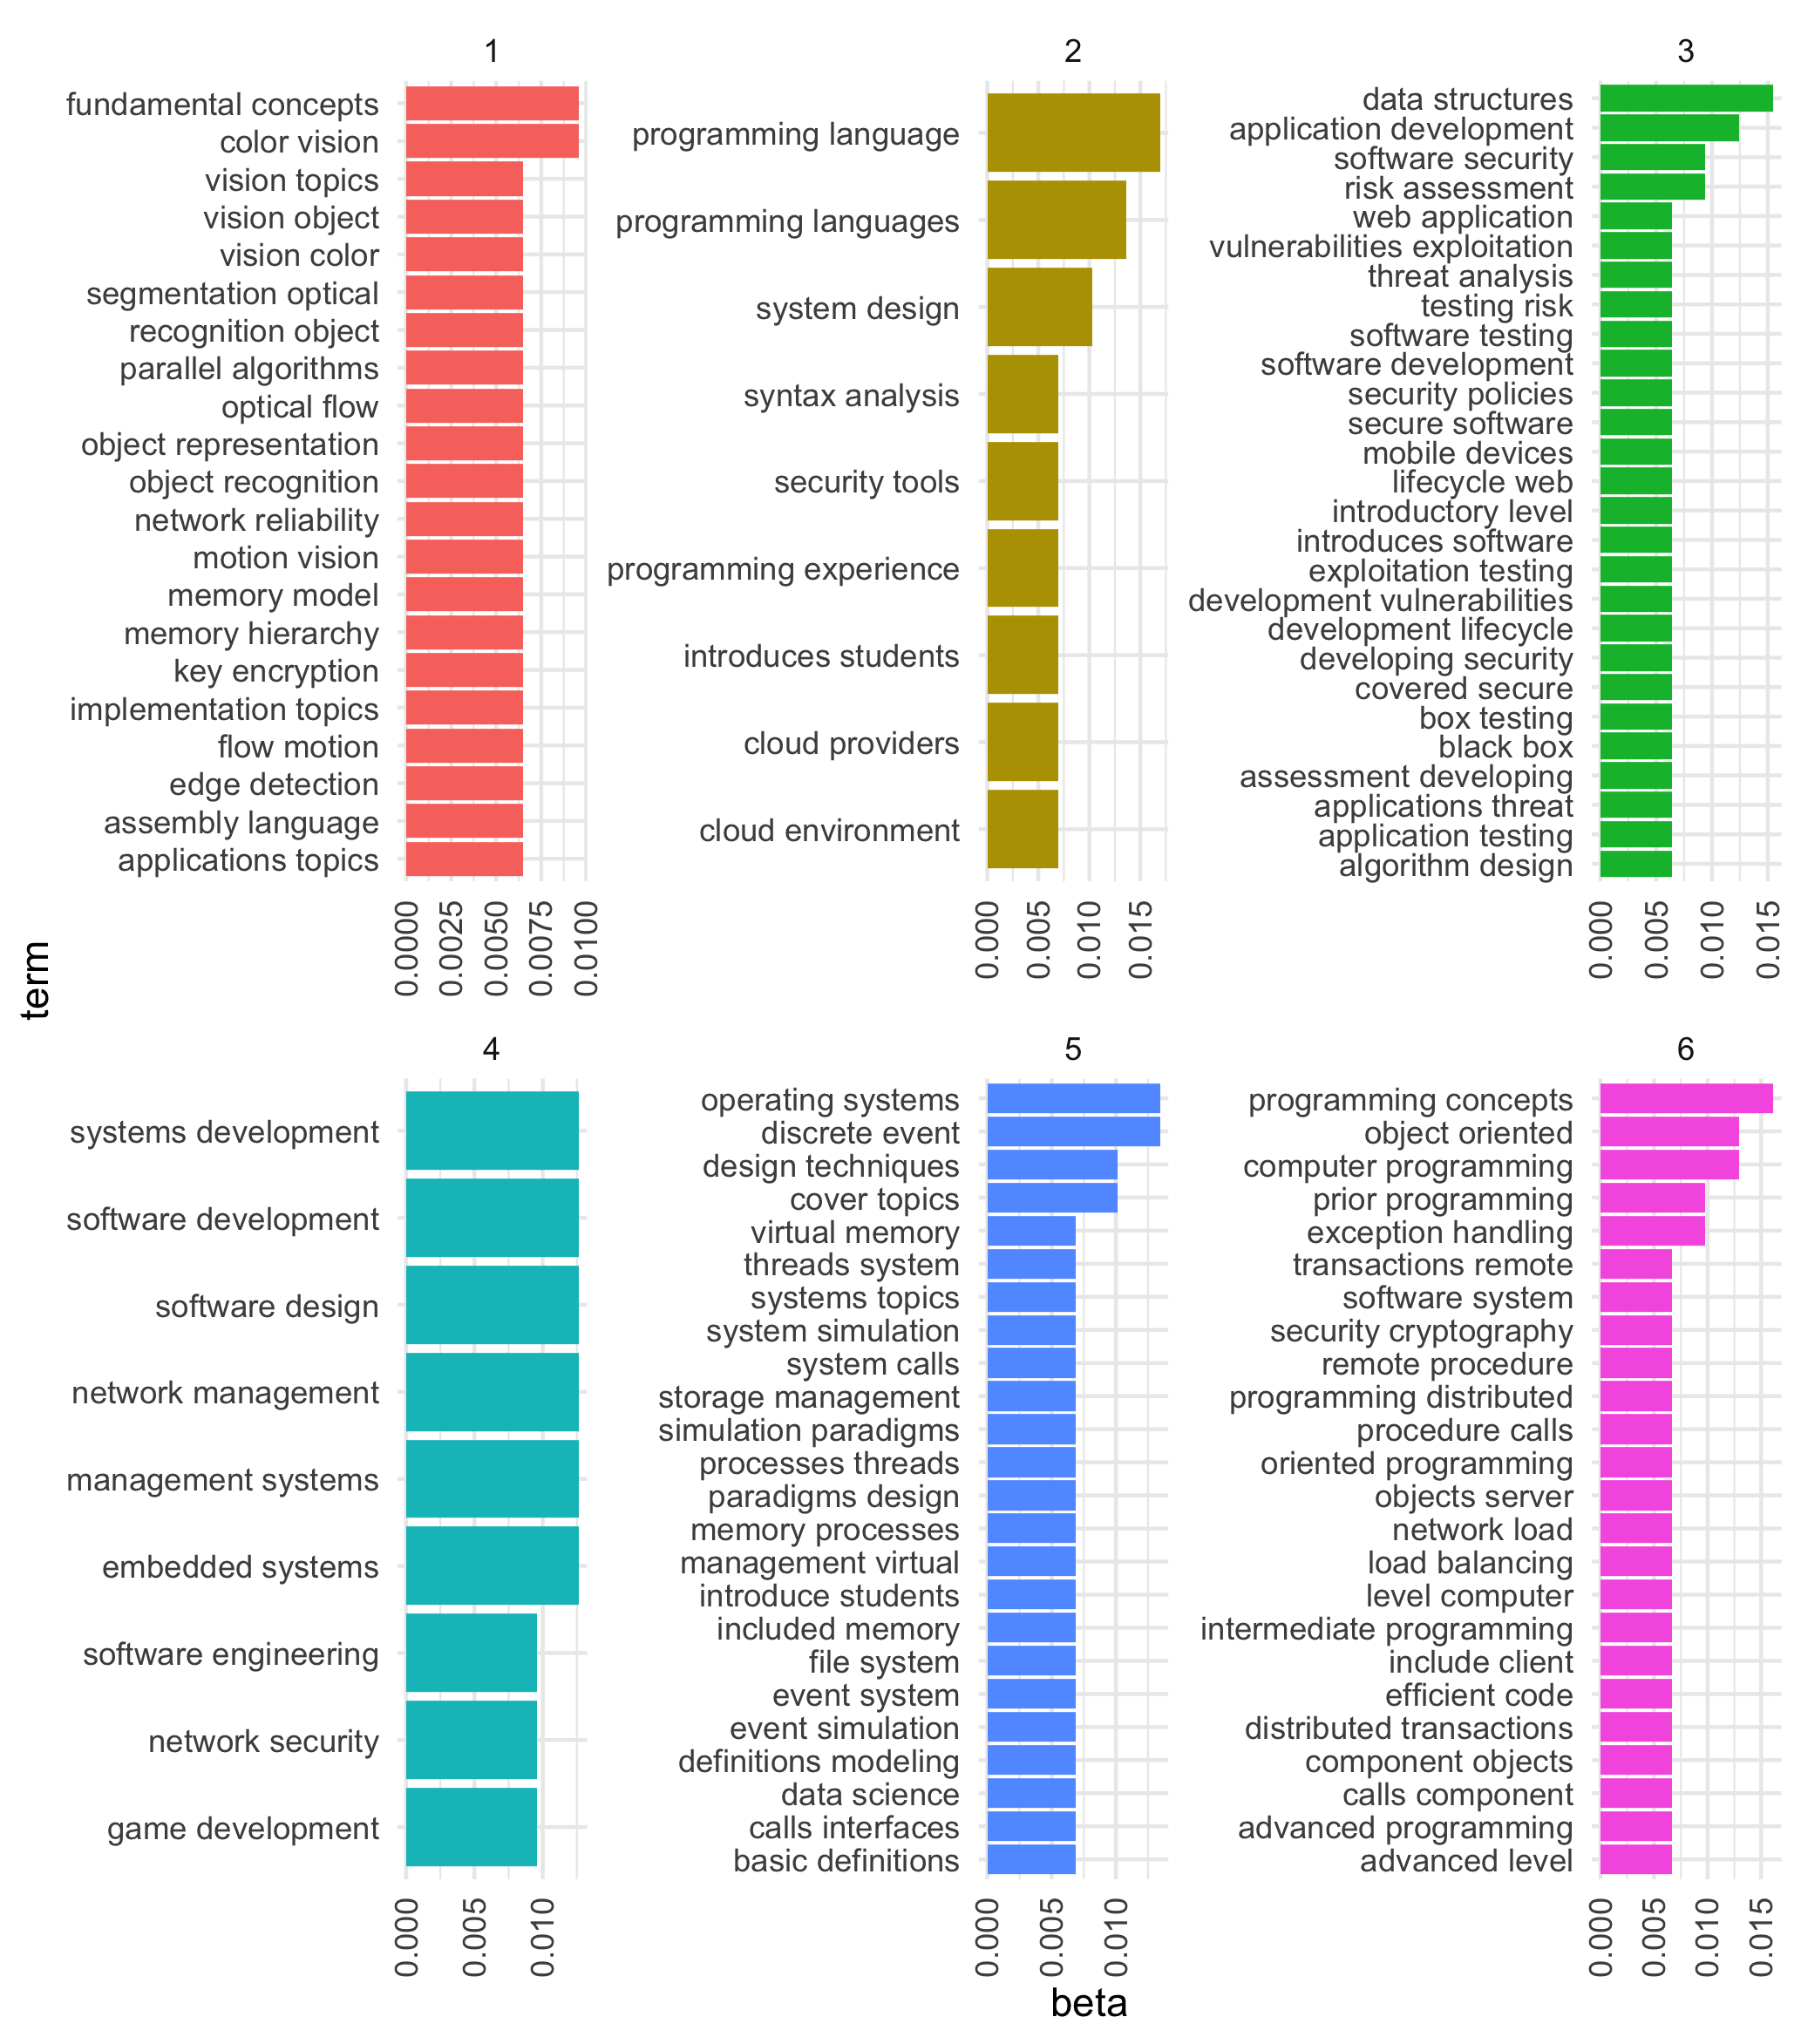
\includegraphics[width = .8\textwidth, height = .7\textheight]{images/lda_cs.png}
  \caption{LDA topic model splitting course topics into concentrations for the Computer Science Plan of Study}
  \label{fig:lda_cs}
\end{figure}

Topic 6 seems to most likely be either Software Engineering or Advanced Topics with terms like "object oriented" and "remote procedure" while topics 2 and 3 fit with Big Data 
Analytics and Cyber Security respectively. Topic 1 has terms that can be aligned with Autonomous Systems like "objection recognition", 
memory model", and "edge detection". 

We can also see how using the cosine similarity works in segmenting the courses based on their full descriptions. Figure \ref{fig:cos_cs} 
shows these results. 

\begin{figure}[H]
  \centering
  
  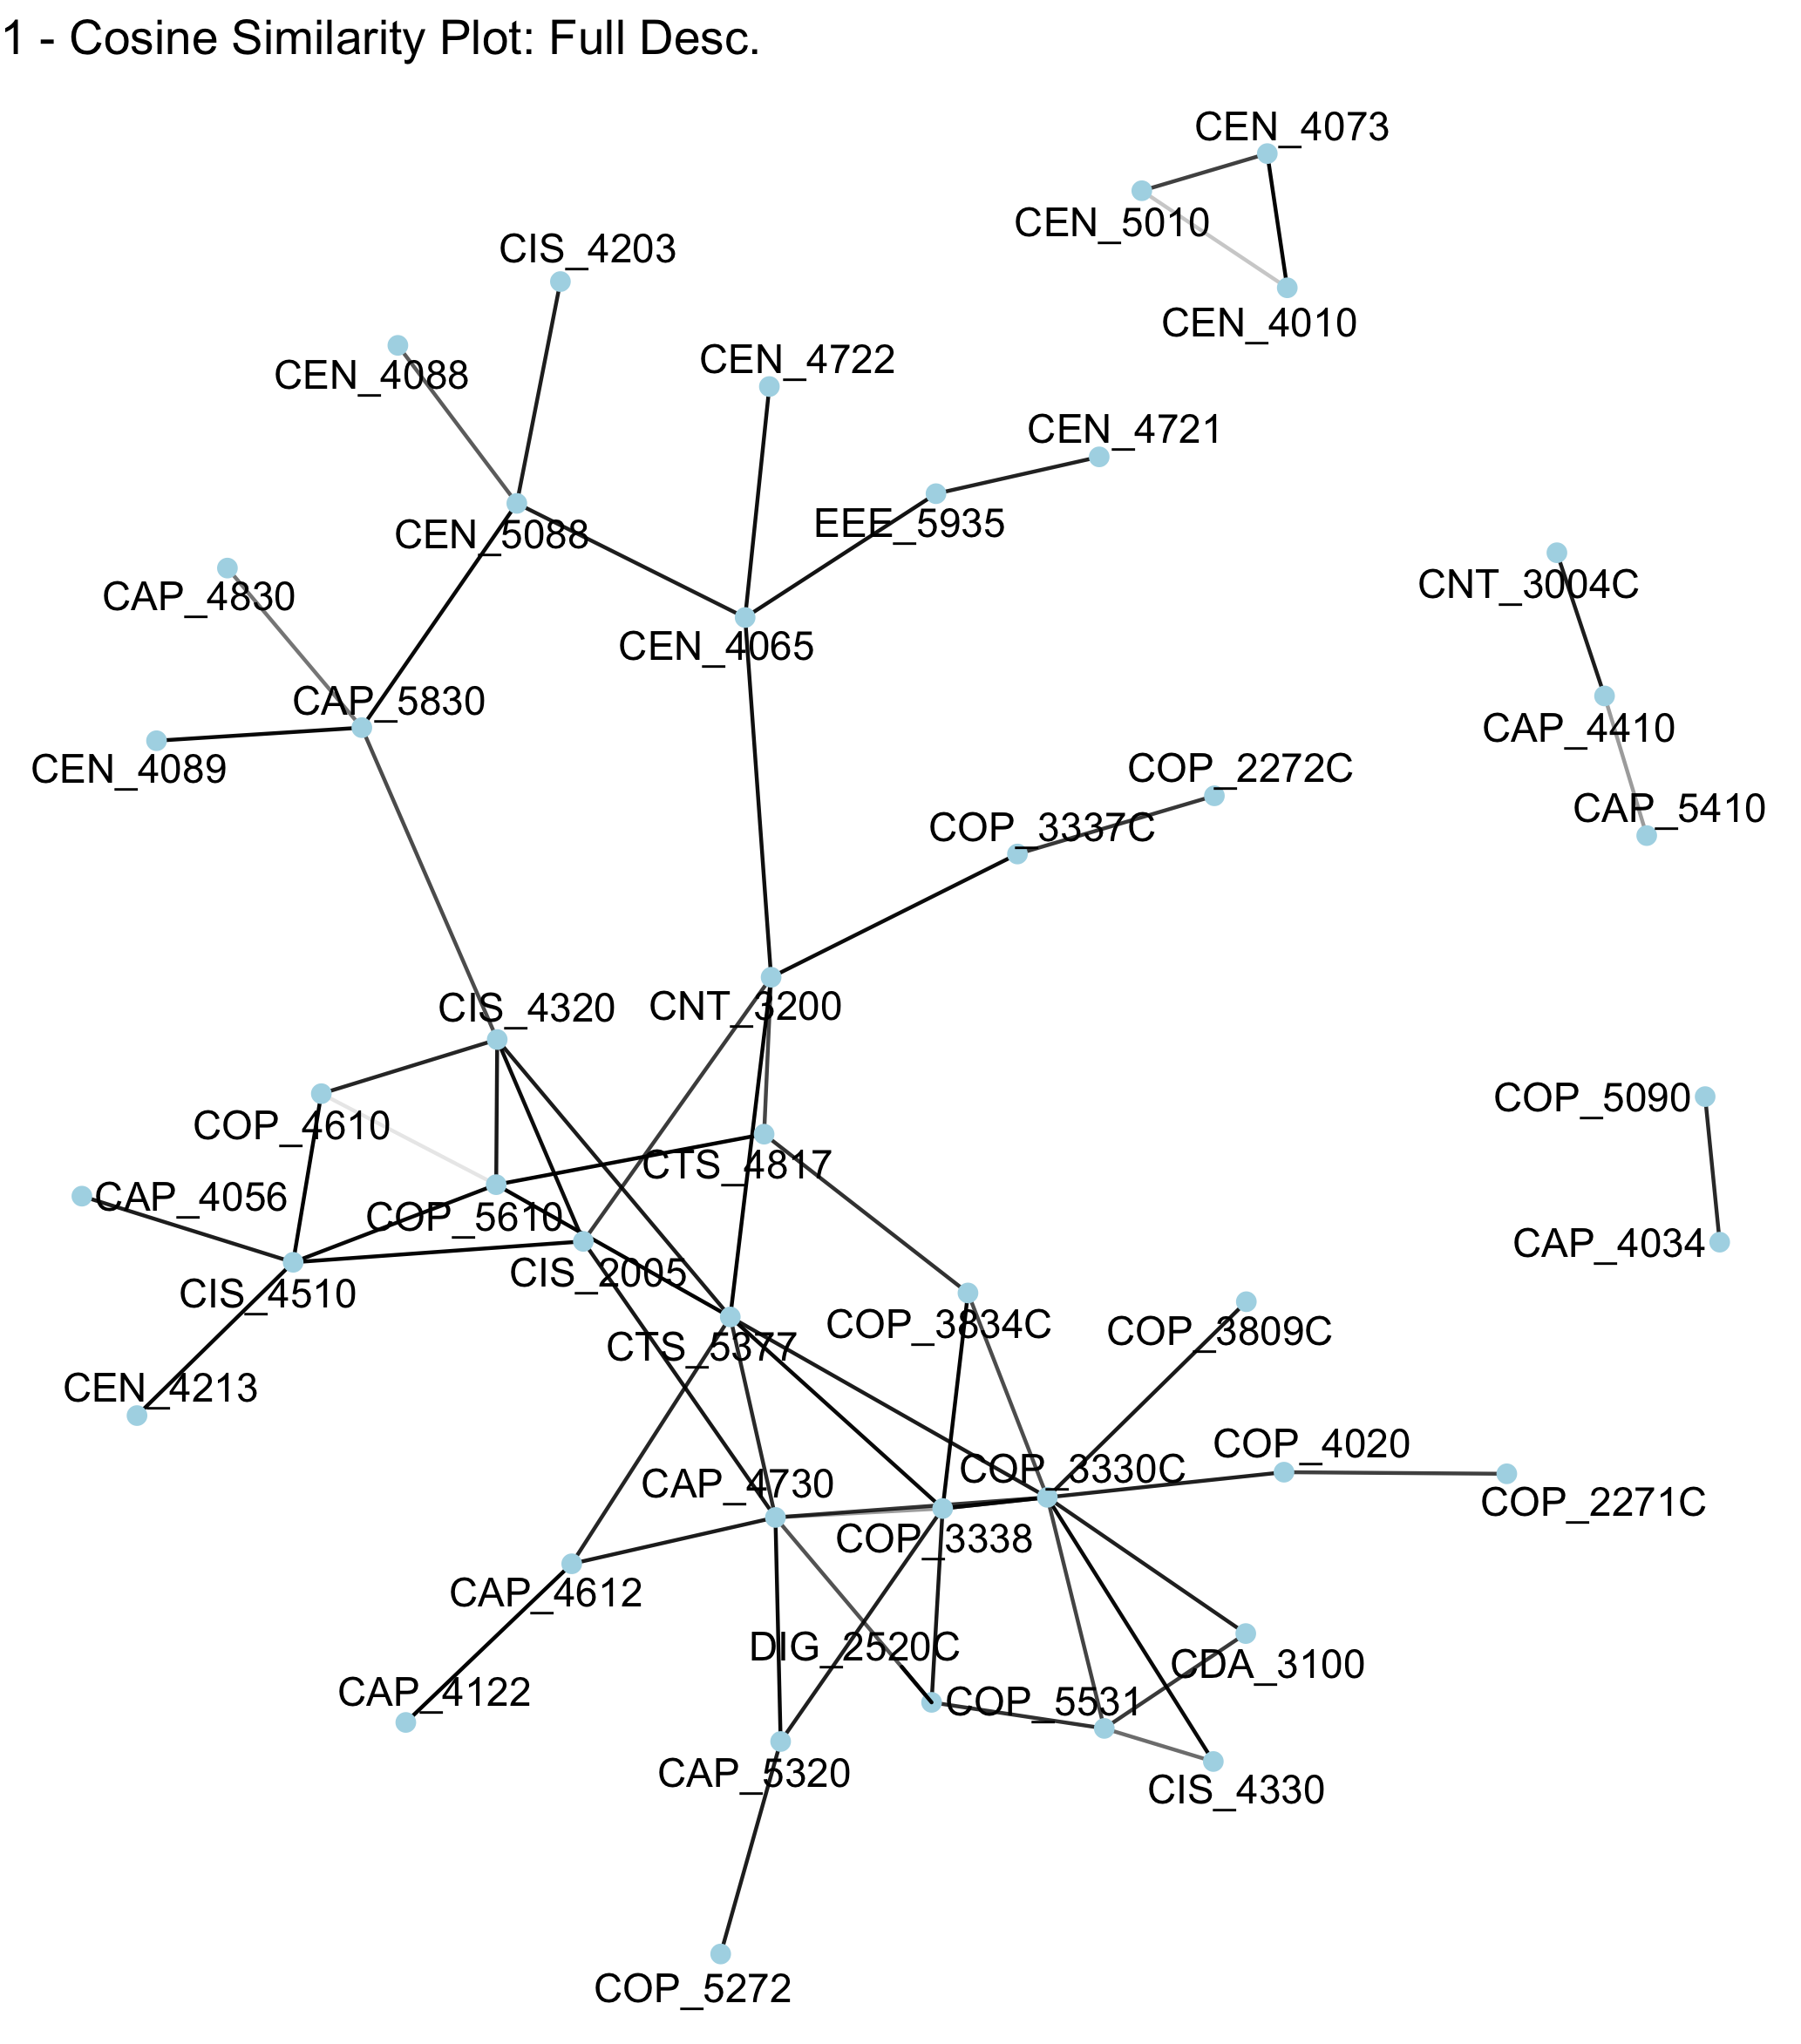
\includegraphics[width = .8\textwidth, height = .7\textheight]{images/cos_cs.png}
  \caption{Cosine distance plot for Computer Science plan of study}
  \label{fig:cos_cs}
\end{figure}

We can see the CEN classes (Software Engineering, Software Design and Architecture, etc.) group together at the top of the plot. 
Where as COP 3330C (Computer Programming 2) Lies at the center of a particularly large grouping at the bottom of the plot. 
This lines up since COP 3330 happens to be either a pre-requisite or co-requisite to the courses it is closest too. The MDS 
biplot can be seen in Figure \ref{fig:cmds_cs}

\begin{figure}[H]
  \centering
  
  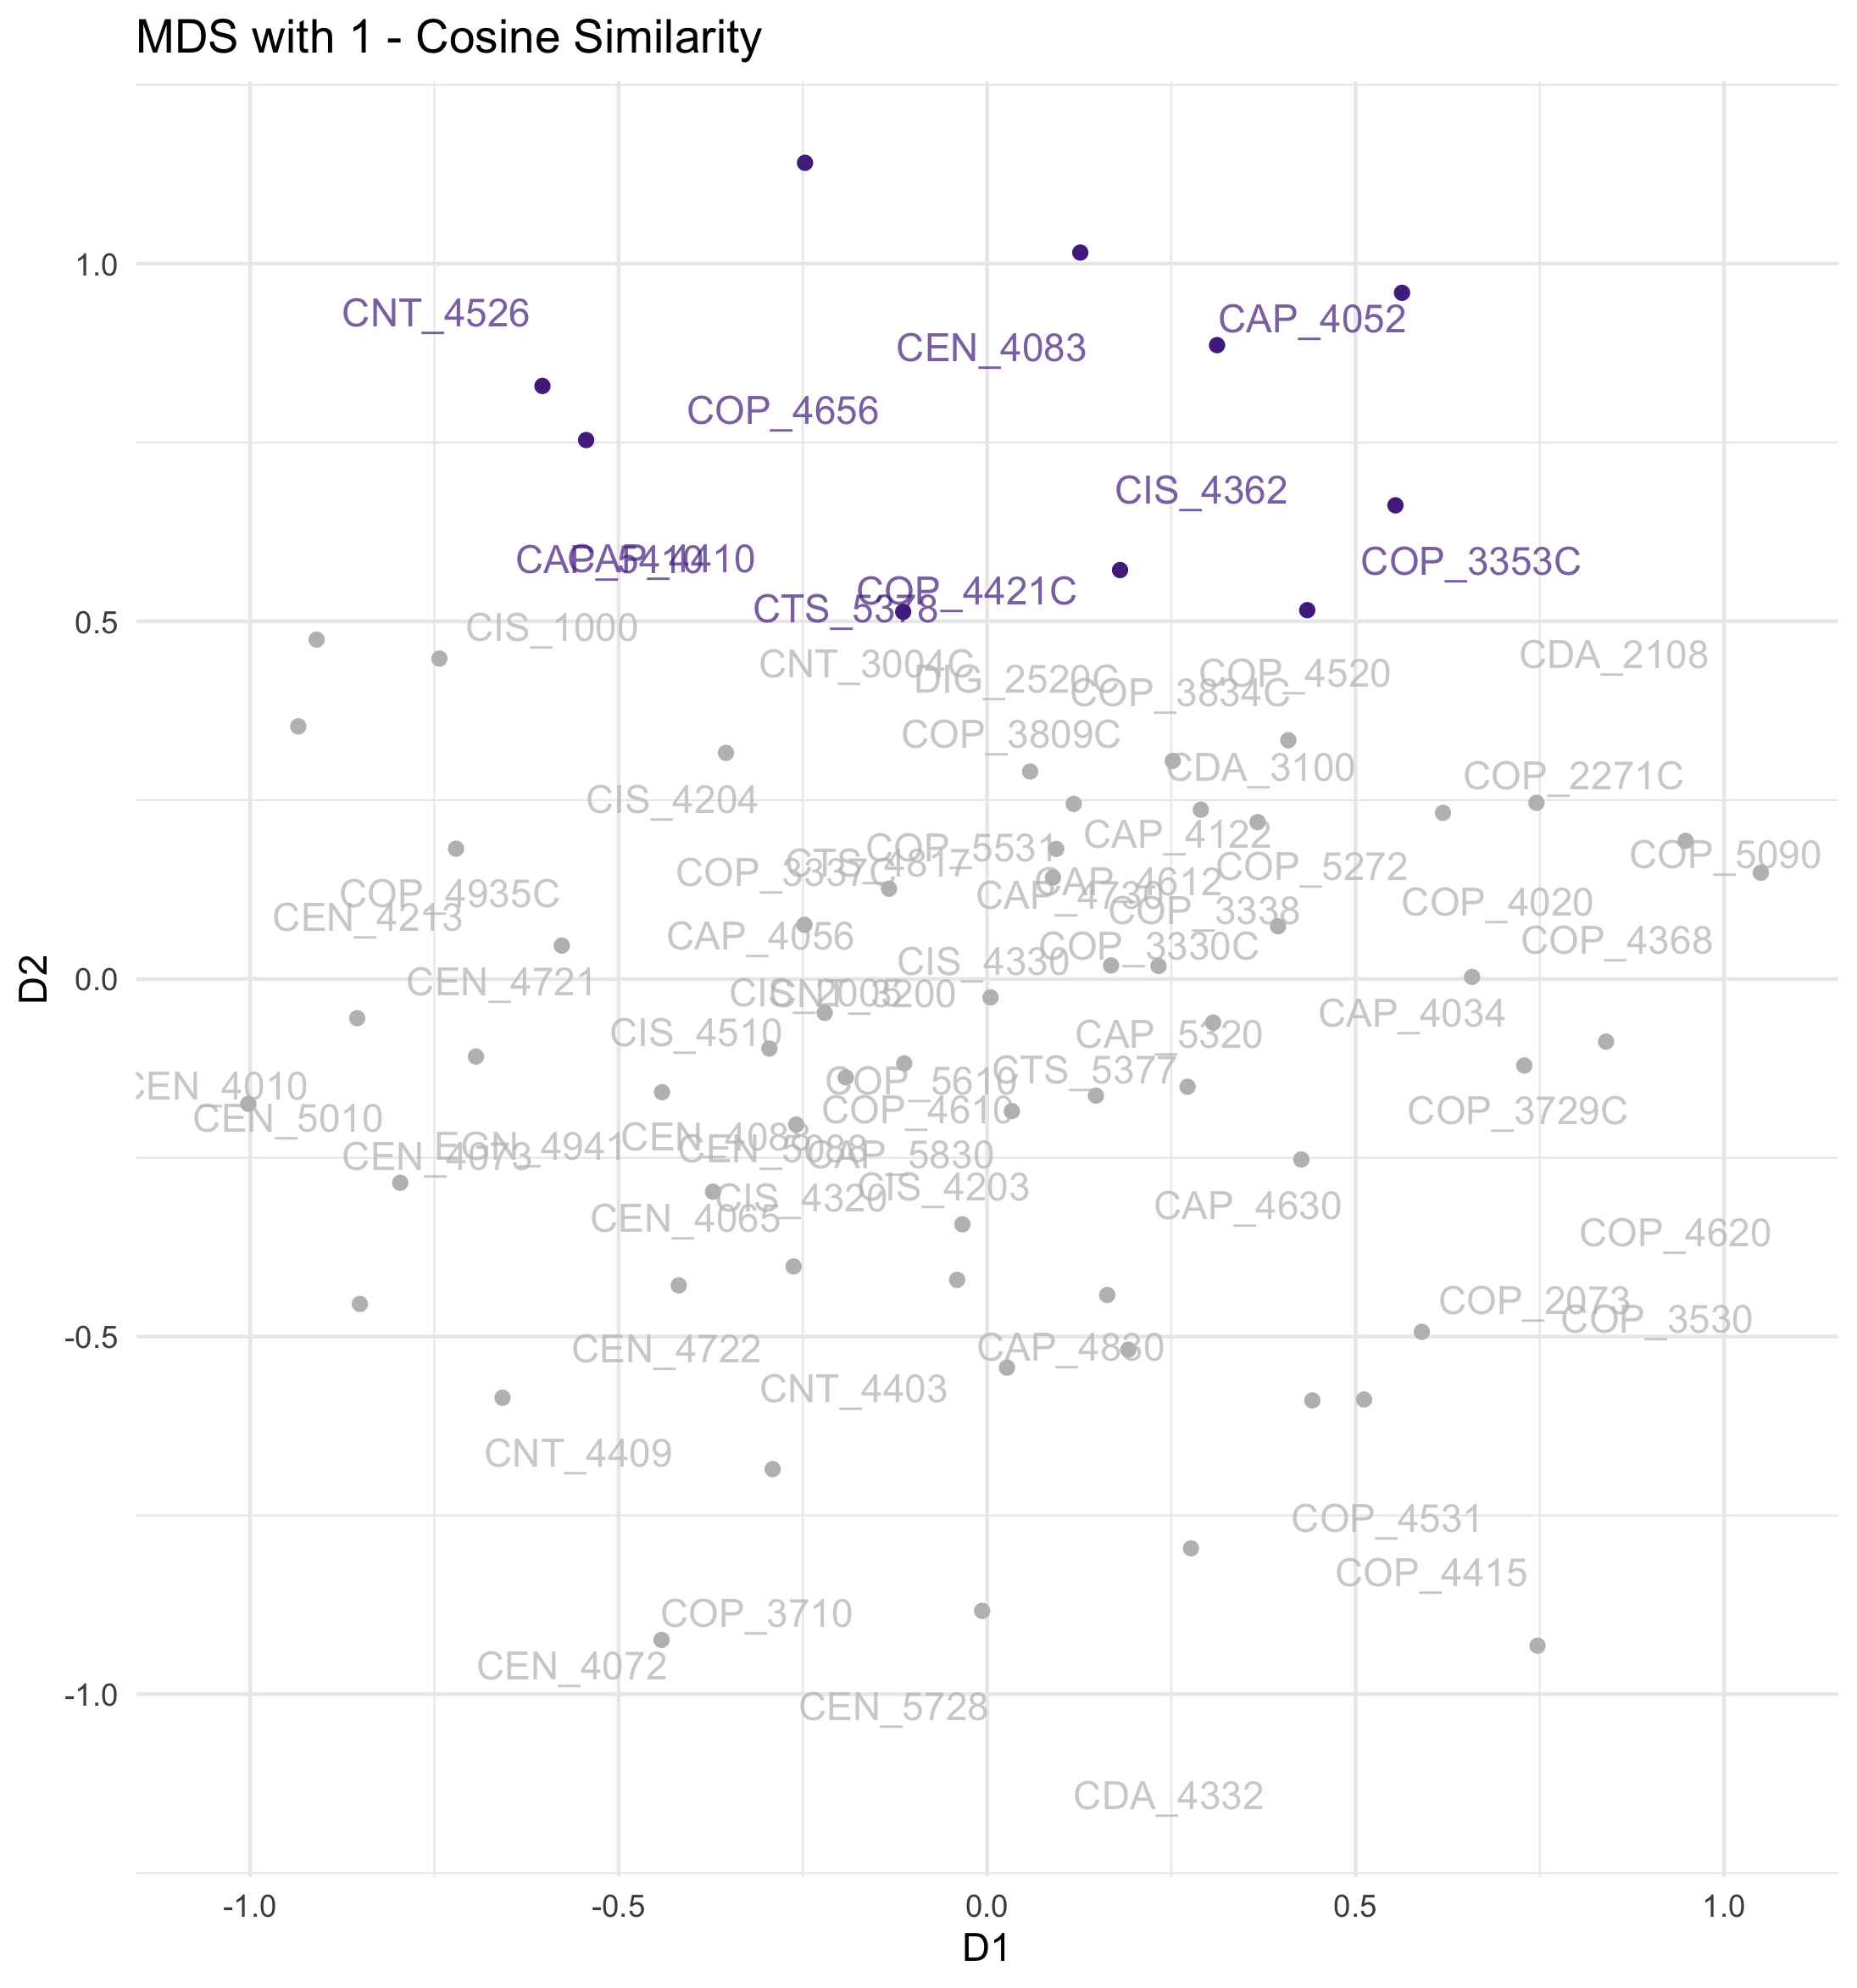
\includegraphics[width = .8\textwidth, height = .7\textheight]{images/cos_mds_cs.png}
  \caption{Cosine distance plot for Computer Science plan of study}
  \label{fig:cmds_cs}
\end{figure}

This results in a much wider distribution across the two latent dimensions from MDS. There seem to be a larger quantity of 
"niche" or non-fundamental classes within CS as a whole, where courses like Advanced Computer Vision (CAP 4410) and 
System Architecture (CDA 4332) can exist toward the outer edges of the catalog. Both of these courses are electives that can be taken 
as concentration courses. 


\section{Research Questions}

\begin{enumerate}

	\item \textit{Are there suggested course topics that can better inform course design/degree design?}

  \vspace{4pt}
From the LDA and the MCA results, it seems as though additional concepts related 
to markets, supply chains,  would have relatively little impact to overall degree design since they already make up a 
majority of the entire DSBA curriculum. Words with smaller betas from the LDA and in more fundamental or "central" 
positions in the MCA seem to be less prevalent, and thus less reinforced through successive coursework. Some of these 
concepts include "uncertainty demand" , "money risk", "economic analysis", "machine learning", "model building",  
and other "information systems" related concepts.

	\item \textit{How can one characterize incremental learning of fundamental topics in a given discipline based on the current curriculum structure?}
	
  \vspace{4pt}
One could possible characterize incremental learning of fundamental topics by mapping student scores on quizzes and exams,
and map the topics mentioned in those questions to the topics in the association graphics shown here \ref{fig:cos}. A 
sufficiently large body of questions should have a large amount of the topics from any given course spread throughout, which 
can display the learning of fundamental topics that tend to "cluster" together in the different graphs. For example, incremental 
learning could be learning fundamental linear algebra principles from a computation class, which when those topics are compared to the course-concept 
association graphs,  the distance of those topics from other "core" topics in the discpline will give a direct measure of how well the material is understood.

	\item \textit{Is there sufficient evidence to develop a case for non-linear course design in degrees?}
\vspace{4pt}

After careful consideration we have determined that additional analysis is needed to provide sufficient evidence to suggest 
non-linear course design. The framework built from the work here may provide sufficient evidence through successive iterations
of the project down the line and its setup facilitates this. 


\end{enumerate}


\section{Conclusion}


Learning Analytics and Unsupervised Learning methods were used as basis for developing course-concept association graphs. 
This work displayed these associations after a preliminary text mining analysis via the creation of document-term matrices 
on course catalog data.  This then evolved into creating clusters using dimensionality reduction methods such as MCA to 
further define course-concept relations, as well as set the groundwork for more  micro-analyses in further iterations by 
creating distance matrices with a variety of distance metrics.  There were numerous interesting takeaways gained from the 
analyses performed here, as well as many different downsides to each approach. However we see the results here as an 
overall positive for future degree design.  Additional analysis is needed to provide sufficient evidence to suggest 
non-linear course design,  however the groundwork is there for future analyses to determine so.

We believe this  project resulted in contributions to the existing body of knowledge on these techniques applied to 
learning analytics, as well as to the University as a whole in providing a tangible body of work to be used by future 
students, faculty, and course planners.   The templates and code produced here can be easily applied to other 
degree programs like Computer Science and Mechanical Engineering by just changing a single line of code. The code 
included also has measures in place for maintaining dependencies reliably,  ensuring that the work is reproducible 
with minimal effort. With Learning Analytics being an emergent field, relevant research to undertake, helping to add 
to the body of knowledge and encouraging the use of modern data-driven curriculum design at Florida Polytechnic University. 

\section{Future Work}
As stated above,  the entire investigation is built on open-source technologies in the R ecosystem with all code published 
to Github. This allows the entire project to be cloned and iterated upon through future explorations of the techniques 
discussed. One specific upside of this is that the code can easily applied to course data from other degree programs at FPU. A simple line of code to a function allows the work here to be applied to any department, with data cleaning and utility functions that can be iterated on. See the appendix below for more.

Some future implementations of this work can include approaches like BERTScores and OK scores as alternative distance 
approaches. Sparse Factor Analysis for an alternative to the network association graph creation. And other non-linear forms of dimensionality reduction.  There is also the potential for this data to be available to students, either through a web application or publicly available GUI for use in course planning for their academic success. 
It would also be feasible to gain data on question-concept association graphs \citep{willcox_network_2017} through sufficiently large databases of questions 
given to students over time that are characterized by the topics covered by those questions. This could potentially link student 
performance to their overall response to plans of study to adjust even further. 


\cleardoublepage

\bibliographystyle{IEEEtran}
\bibliography{project-proposal}

\cleardoublepage

\renewcommand\appendixpagename{Appendix}
\appendix
%\appendixpagename

%\addappheadtotoc


\titleformat{\chapter}{\normalfont\LARGE\scshape}{Appendix \thechapter: }{.1em}{\vspace{1ex}}[\titlerule]
% appendixes go here
\begin{appendices}
\chapter{Glossary}
  \begin{itemize}
    \item{Unsupervised Learning: the use of algorithms on unlabeled data to obtain clusters, or groupings, that partition the data.}
  
    \item{Supervised Learning: the use of algorithms on labeled data to classify (or regress) data into categories (or estimate values).}
  
    \item{Bigram/N-Gram: a pair of two words which appear adjacent to one another in text. Generalized to $n$ words appearing adjacent to one another, in sequence.}

  \end{itemize}
\chapter{Session Info - R}

\begin{lstlisting}
> sessionInfo()
R version 4.0.3 (2020-10-10)
Platform: x86_64-apple-darwin19.6.0 (64-bit)
Running under: macOS Big Sur 10.16

Matrix products: default
LAPACK: /usr/local/Cellar/r/4.0.3/lib/R/lib/libRlapack.dylib

locale:
[1] en_US.UTF-8/en_US.UTF-8/en_US.UTF-8/C/en_US.UTF-8/en_US.UTF-8

attached base packages:
[1] stats     graphics  grDevices datasets  utils     methods   base     

other attached packages:
 [1] slam_0.1-47              topicmodels_0.2-11       ggraph_2.0.4             igraph_1.2.6             widyr_0.1.4             
 [6] stringdist_0.9.8         ggrepel_0.8.2            smacof_2.1-3             e1071_1.7-9              colorspace_2.0-2        
[11] plotrix_3.8-2            proxy_0.4-26             broom_0.7.10             textmineR_3.0.5          Matrix_1.3-4            
[16] SparseFactorAnalysis_1.0 proto_1.0.0              directlabels_2021.1.13   plotly_4.10.0            factoextra_1.0.7        
[21] FactoMineR_2.3           tm_0.7-8                 NLP_0.2-1                tidytext_0.3.2           tidyr_1.1.4             
[26] DT_0.16                  stringr_1.4.0            purrr_0.3.4              readr_1.4.0              dplyr_1.0.7             
[31] ggplot2_3.3.5            here_1.0.1              

loaded via a namespace (and not attached):
  [1] backports_1.4.0      Hmisc_4.6-0          VGAM_1.1-5           plyr_1.8.6           lazyeval_0.2.2       splines_4.0.3       
  [7] crosstalk_1.2.0      SnowballC_0.7.0      candisc_0.8-6        digest_0.6.28        foreach_1.5.1        htmltools_0.5.2     
 [13] viridis_0.6.2        gdata_2.18.0         fansi_0.5.0          magrittr_2.0.1       checkmate_2.0.0      cluster_2.1.2       
 [19] doParallel_1.0.16    graphlayouts_0.7.1   wordcloud_2.6        jpeg_0.1-9           xfun_0.28            crayon_1.4.2        
 [25] jsonlite_1.7.2       lme4_1.1-27.1        survival_3.2-13      iterators_1.0.13     glue_1.5.0           polyclip_1.10-0     
 [31] stopwords_2.3        gtable_0.3.0         nnls_1.4             car_3.0-12           weights_1.0.4        abind_1.4-5         
 [37] scales_1.1.1         rstatix_0.6.0        Rcpp_1.0.7           viridisLite_0.4.0    htmlTable_2.3.0      flashClust_1.01-2   
 [43] foreign_0.8-81       Formula_1.2-4        stats4_4.0.3         heplots_1.3-9        truncnorm_1.0-8      htmlwidgets_1.5.4   
 [49] httr_1.4.2           RColorBrewer_1.1-2   modeltools_0.2-23    ellipsis_0.3.2       mice_3.13.0          pkgconfig_2.0.3     
 [55] farver_2.1.0         nnet_7.3-16          utf8_1.2.2           tidyselect_1.1.1     labeling_0.4.2       rlang_0.4.12        
 [61] reshape2_1.4.4       polynom_1.4-0        munsell_0.5.0        tools_4.0.3          cli_3.1.0            generics_0.1.1      
 [67] evaluate_0.14        fastmap_1.1.0        yaml_2.2.1           knitr_1.36           tidygraph_1.2.0      nlme_3.1-153        
 [73] leaps_3.1            xml2_1.3.2           tokenizers_0.2.1     compiler_4.0.3       rstudioapi_0.13      png_0.1-7           
 [79] ggsignif_0.6.0       tweenr_1.0.1         tibble_3.1.6         stringi_1.7.5        lattice_0.20-45      nloptr_1.2.2.3      
 [85] vctrs_0.3.8          pillar_1.6.4         lifecycle_1.0.1      data.table_1.14.2    R6_2.5.1             latticeExtra_0.6-29 
 [91] renv_0.14.0          RcppProgress_0.4.2   gridExtra_2.3        janeaustenr_0.1.5    codetools_0.2-18     boot_1.3-28         
 [97] MASS_7.3-54          gtools_3.9.2         rprojroot_2.0.2      withr_2.4.2          parallel_4.0.3       hms_0.5.3           
[103] quadprog_1.5-8       grid_4.0.3           rpart_4.1-15         class_7.3-19         minqa_1.2.4          rmarkdown_2.11      
[109] carData_3.0-4        ggpubr_0.4.0         ggforce_0.3.2        scatterplot3d_0.3-41 base64enc_0.1-3      ellipse_0.4.2       
\end{lstlisting}

\chapter{Example Code} 

\begin{lstlisting}
\# Calculating the cosine similarity/distance matrix
cos_mat <- stringdistmatrix(course_full_desc$text, course_full_desc$text, 
useNames = FALSE, method = "cosine") %>% 
  as.matrix()

colnames(cos_mat) <- course_full_desc$Course_ID
rownames(cos_mat) <- course_full_desc$Course_ID

cos_course <- reshape2::melt(cos_mat)[reshape2::melt(upper.tri(cos_mat))$value,]

colnames(cos_course) <- c("Term1", "Term2", "distance")


# Plotting 
cos_course %>% 
  filter(distance < 0.02) %>% 
  graph_from_data_frame() %>%
  ggraph(layout = "fr") +
  geom_edge_link(aes(edge_alpha = distance), show.legend = FALSE) +
  geom_node_point(color = "lightblue", size = ptsize) +
  geom_node_text(aes(label = name), repel = TRUE) +
  theme_void() + 
  labs(title = "1 - Cosine Similarity Plot: Full Desc.")

ggsave("img/cos.png", dpi = 300)


# Calculating the Jaccard similarity/distance matrix
jac_mat <- stringdistmatrix(course_full_desc$text, course_full_desc$text, useNames = FALSE, method = "jaccard") %>% 
  as.matrix()

colnames(jac_mat) <- course_full_desc$Course_ID
rownames(jac_mat) <- course_full_desc$Course_ID

jac_course <- reshape2::melt(jac_mat)[reshape2::melt(upper.tri(jac_mat))$value,]

colnames(jac_course) <- c("Term1", "Term2", "distance")

# Plotting
jac_course %>% 
  filter(distance < 0.04) %>% 
  graph_from_data_frame() %>%
  ggraph(layout = "fr") +
  geom_edge_link(aes(edge_alpha = distance), show.legend = FALSE) +
  geom_node_point(color = "lightblue", size = ptsize) +
  geom_node_text(aes(label = name), repel = TRUE) +
  theme_void() + 
  labs(title = "1 - Jaccard Similarity Plot: Full Desc.")

ggsave("img/jac.png", dpi = 300)

# MDS
mds_cos_mat <- cos_mat %>% 
  mds(type = "ordinal")

ggplot() +
  geom_point(data = as_tibble(mds_cos_mat$conf), aes(x = D1, y = D2, 
  colour = D2 > 0.5)) +
  scale_colour_manual(values = setNames(c('#532d8e','grey'),c(T, F))) +
  scale_alpha_manual(values = c(1, 0.01)) +
  geom_text(as_tibble(mds_cos_mat$conf), mapping = aes(
    x = -D1, y = -D2, color = D2 < -0.5, label = paste(rownames(cos_mat))), alpha = .7) +
  geom_text_repel() +
  theme_minimal() +
  labs(title = "MDS with 1 - Cosine Similarity") +
  theme(legend.position = "")

ggsave("img/cos_mds.png", dpi = 300) 

# Fitting an LDA topic model
# k = 5 for the number of concentrations
bigram_lda <- LDA(bigram_dtm, k = 5, method = "Gibbs", control=list(iter = 500, verbose = 25, alpha = 0.2))
 

\end{lstlisting}

\chapter{Mechanical Engineering and Environmental Engineering Plan of Study}

Mechanical Engineering and Environmental Engineering has less programming courses and emphasizes more math related courses. Again, we fit a topic model 
to find the number of concentrations (k = 5). Figure \ref{fig:lda_me} shows the model's performance on this plan of study. Here is a list of the concentrations:

\begin{itemize}
  \item Advanced Topics
  \item Aerospace Engineering
  \item Materials and Advanced Manufacturing
  \item Mechanical and Thermal Systems
  \item Operations Research 
\end{itemize}

\begin{figure}[H]
  \centering
  
  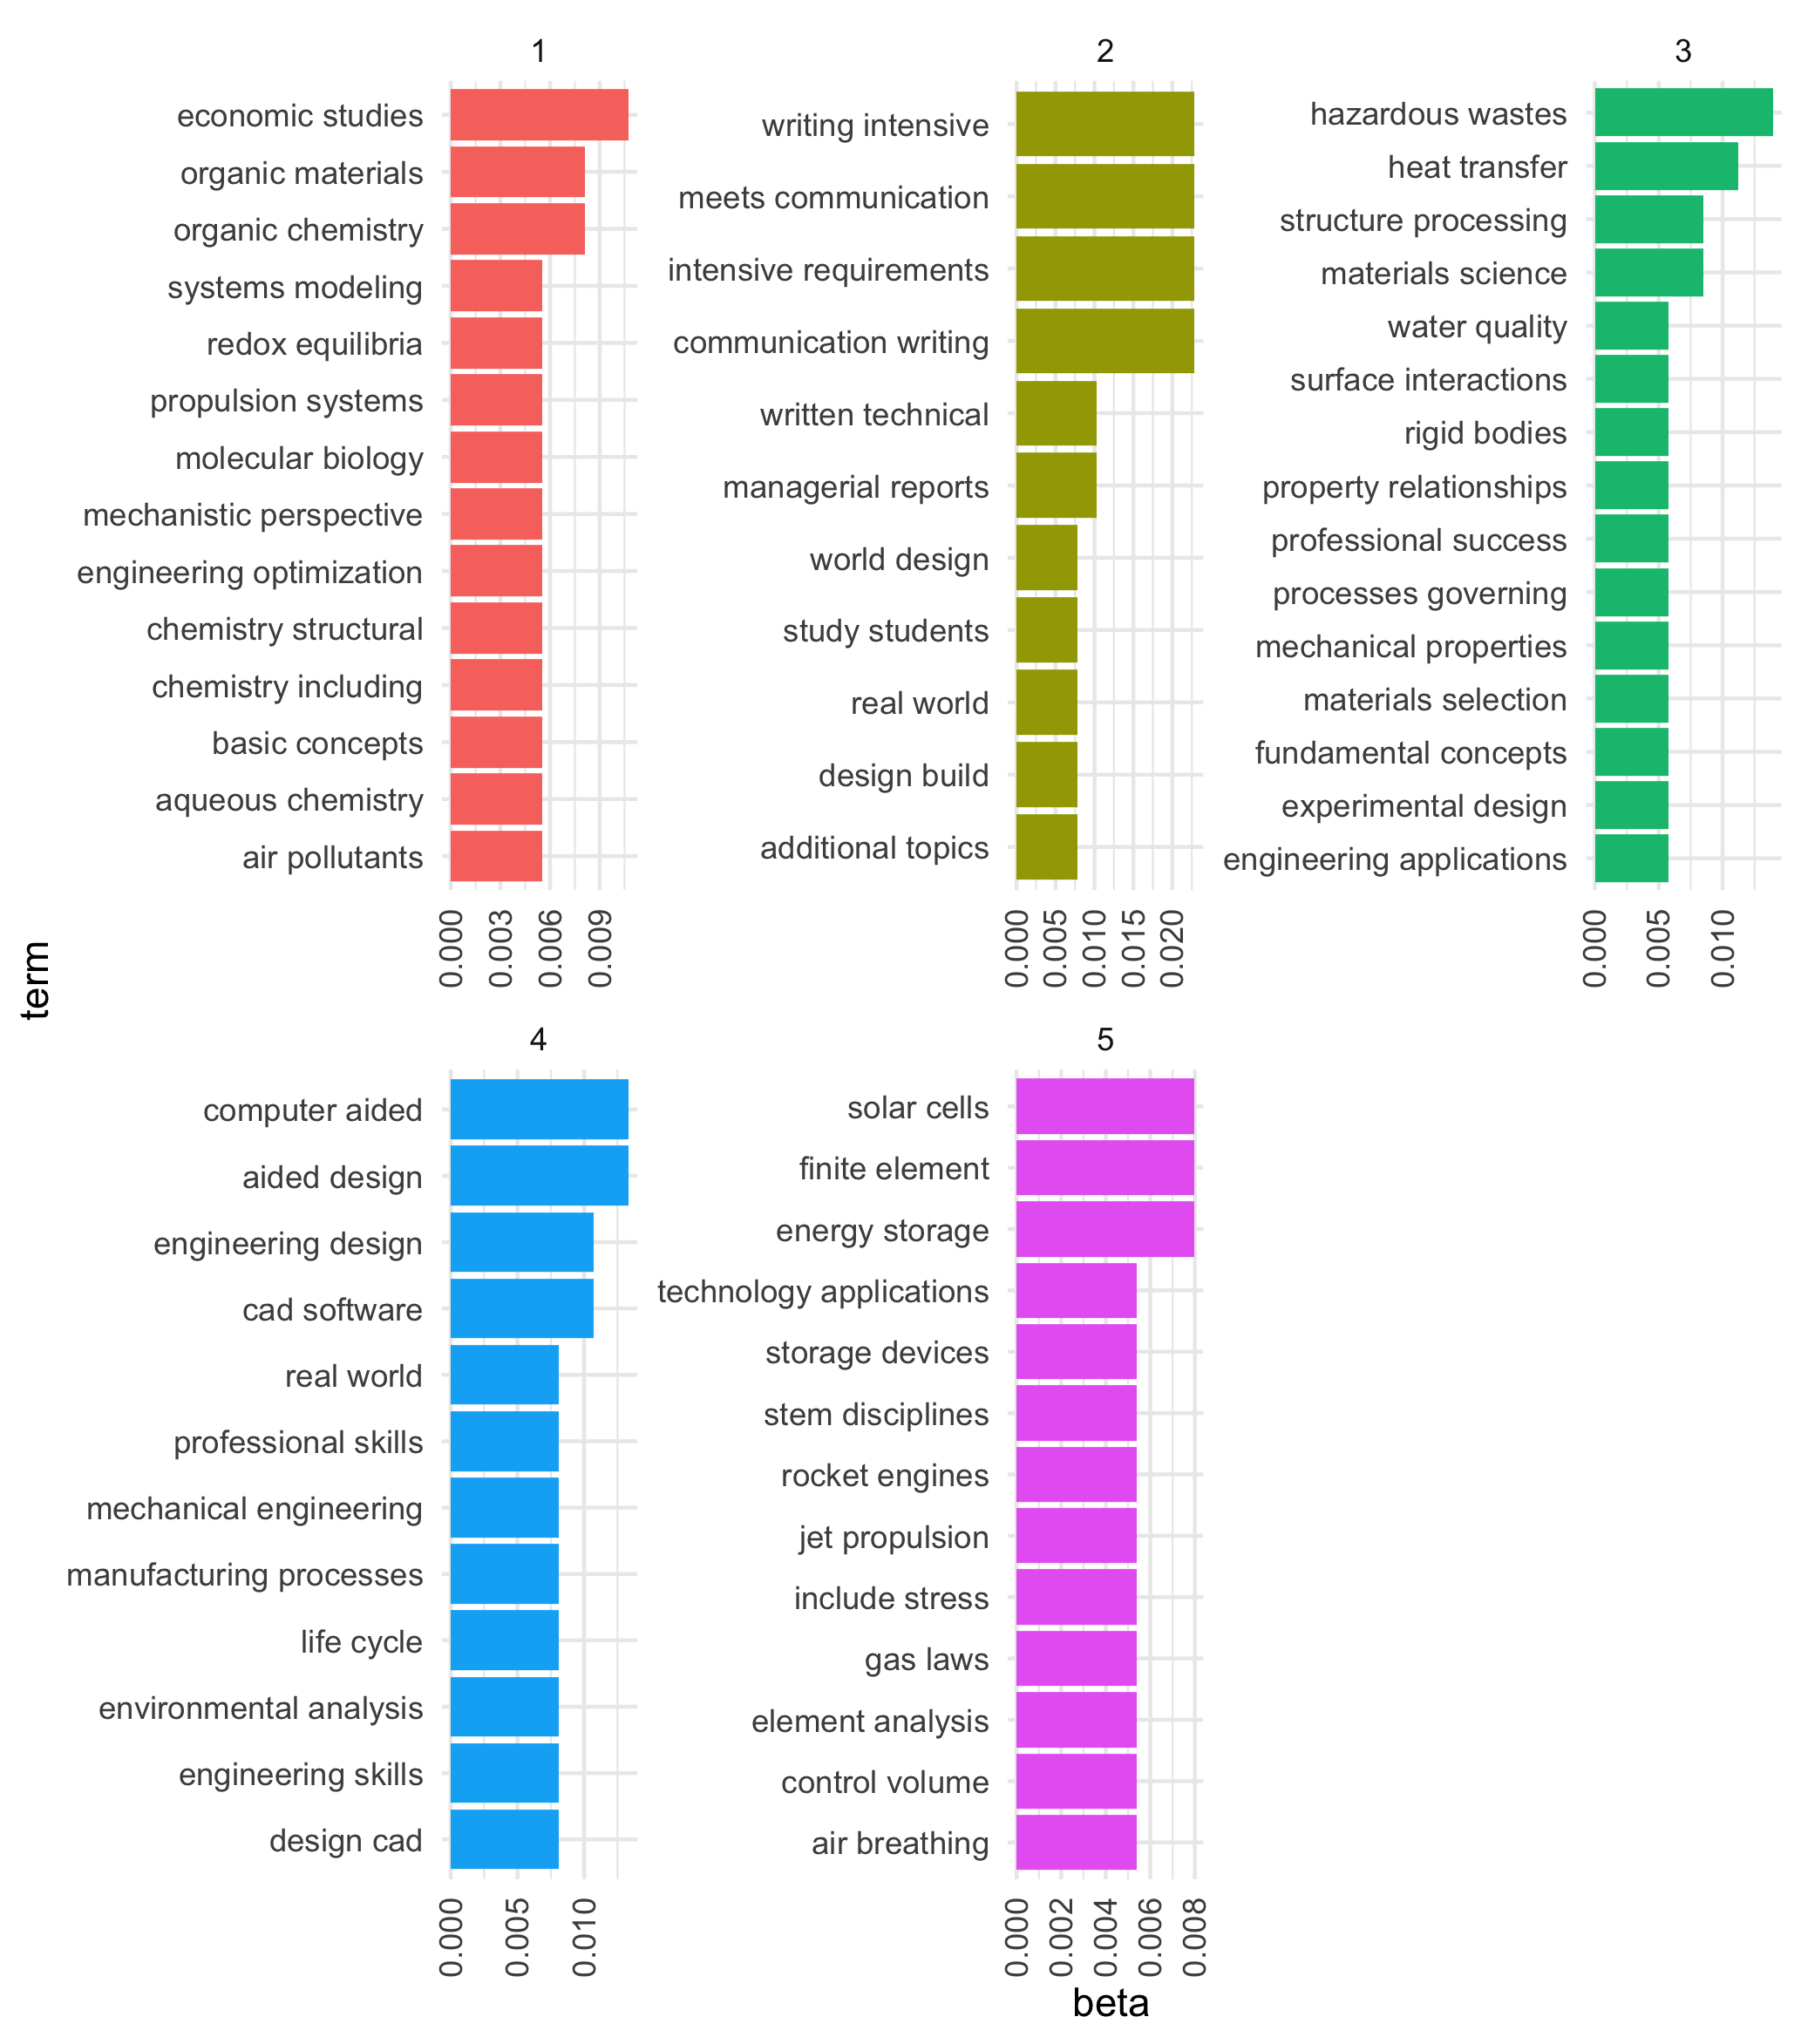
\includegraphics[width = .8\textwidth, height = .7\textheight]{Content/images/lda_me.png}
  \caption{LDA topic model splitting course topics into concentrations for the Mechanical Engineering Plan of Study}
  \label{fig:lda_me}
\end{figure}

\end{appendices}


\end{document}